\documentclass[11pt,a4paper]{article}

% ---------------------------------------------------------------------------
% Packages
% ---------------------------------------------------------------------------
\usepackage[utf8]{inputenc}
\usepackage[T1]{fontenc}
\usepackage{lmodern}
\usepackage[margin=1in]{geometry}
\usepackage{amsmath,amssymb,amsthm}
\usepackage{booktabs}
\usepackage{graphicx}
\usepackage{xcolor}
\usepackage{caption}
\usepackage{subcaption}
\usepackage{microtype}
\usepackage[colorlinks=true,linkcolor=blue!50!black,citecolor=blue!50!black,urlcolor=blue!50!black]{hyperref}
\usepackage{enumitem}
\usepackage{tabularx}
\usepackage{array}
\usepackage[round,authoryear]{natbib}

\setlength{\parindent}{0pt}
\setlength{\parskip}{6pt plus 1pt minus 1pt}

\graphicspath{{figures/}}

% Custom commands. (Note: \Pr is already standard in LaTeX as
% \operatorname{Pr}, so we don't redefine it.)
\newcommand{\E}{\mathbb{E}}
\newcommand{\Var}{\operatorname{Var}}
\newcommand{\VaR}{\operatorname{VaR}}
\newcommand{\ES}{\operatorname{ES}}
\newcommand{\GPD}{\mathrm{GPD}}
\newcommand{\Poi}{\mathrm{Poisson}}
\newcommand{\NB}{\mathrm{NB}}

% ---------------------------------------------------------------------------
% Title
% ---------------------------------------------------------------------------
\title{\textbf{Pricing the DeFi Tail:\\
A Loss-Distribution Approach to Operational-Risk Capital}}

\author{Nils Bundi\\
\small Zurich University of Applied Sciences\\
\small \texttt{nbundi@proton.me}}
\date{Working draft\ \textemdash\ 2026-05-23}

% ---------------------------------------------------------------------------
\begin{document}
\maketitle

\begin{abstract}
\noindent
DeFi disintermediates financial services by outsourcing critical
functions --- custody, settlement, counterparty credit --- and
their associated risks to smart-contract code. Operational risks,
however, remain inside the system and are expressing themselves
in aggregate gross losses of \textbf{USD~11.2~billion across
1{,}495 deduplicated events on DeFi protocols since 2020}.
Basel~III requires banks to hold capital reserves against
operationally analogous losses. DeFi protocols maintain similar
buffers --- Aave's Umbrella safety module, MakerDAO's surplus
buffer, Compound's reserve factor --- but those buffers are
sized today by governance vote and depositor demand, not by
empirical loss data. This paper performs the calibration.

I assemble a deduplicated event-level dataset from seven public
sources covering 2020--2026, tagged against the Basel~III Level-1
operational-risk event-type taxonomy. Fitted peaks-over-threshold
generalised-Pareto severity gives per-sector tail-shape parameters
$\hat\xi$ in $[0.30, 0.93]$ across Stablecoin, Lending, DEX, Yield,
and Bridge: Lending sits just below the infinite-mean boundary
$\hat\xi=0.93$ and is statistically indistinguishable from
\citet{Moscadelli2004}'s canonical Basel~II banking
operational-risk range; the other sectors fit in the moderate-heavy
range. A compound Poisson--GPD loss-distribution Monte Carlo
translates the per-sector severity and frequency primitives into
operational-risk capital ratios expressed as basis points of
protocol TVL: a protocol cannot lose more than its own users
supplied, so the per-sector $\ES_{99\%}/$TVL ratio is the
operationally binding capital target applied protocol-by-protocol.
Per-sector $\ES_{99\%}$ ratios range from $\approx 2{,}000$~bps
(DEX, Bridge, Yield) to $\approx 3{,}800$~bps (Lending) of
protocol TVL. Applied to Aave V3's $\sim$USD~30~B of supplied
lending TVL, this implies a modelled $\ES_{99\%}$ on the order of
USD~11~B against on-chain Umbrella stake currently in the
USD~100--500~m range ---
two orders of magnitude below the modelled tail. MakerDAO's
surplus buffer covers roughly $5\%$ of the modelled Maker-share
requirement; Compound's reserve factor a similar fraction. For
the long tail of DeFi protocols that maintain no formal capital
buffer at all, the same numbers price a stand-alone protocol
insurance cover. The per-sector and per-protocol figures give
protocol teams, depositors, and underwriters a quantitative
reference for sizing DeFi operational-risk capital on the same
statistical basis that banking regulators use.
\end{abstract}

\vspace{4pt}
\hrule
\vspace{4pt}

\textbf{Keywords:} operational risk; extreme value theory; loss
distribution approach; capital requirements; decentralized finance;
smart-contract OpRisk events; tail risk; expected shortfall; Aave
Umbrella; MakerDAO surplus buffer.

% ===========================================================================
\section{Introduction}
% ===========================================================================

Decentralized finance (DeFi) is built around a deliberate
elimination of several risks that dominate the bank balance sheet.
Smart-contract execution on a public blockchain replaces the bank's
custody function: assets are held by code, not by a custodian whose
solvency could collapse \citep{Schar2021}. Settlement is atomic and
verifiable on-chain, eliminating the Herstatt-style cross-currency
settlement risk and the principal-against-payment delays that
traditional clearing infrastructure manages with collateral
deposits and central counterparties. Counterparty credit risk is
collapsed into the overcollateralisation requirement embedded in
the lending or derivatives contract \citep{Werner2022,Auer2024}.
And the rehypothecation chains that complicate prime-broker books
do not exist: every position is identifiable down to the contract
address. These structural risk-eliminations are the substance of the
``trustless'' framing in the DeFi literature
\citep{Schar2021,Werner2022,Auer2024} and explain why the dominant
academic framings of DeFi are either \emph{financial} (market
microstructure, price formation, liquidity) or \emph{security}
(bug taxonomies, formal verification, post-mortem analyses).

What neither framing covers is the residual category. The risks
DeFi keeps --- and in some cases concentrates --- are the
operational ones: external attacks on smart-contract code,
insider-rugpull / internal-fraud events, oracle and economic-design
manipulation, configuration and deployment errors, infrastructure
failures. \citet{Aramonte2021} flag this point as the
``decentralisation illusion'' in their BIS Quarterly Review note:
custody and settlement risk are removed, but operational risk is
not, and the dominant attack surface (the contract code, the
upgrade keys, the oracle, the bridge) is what carries the entire
loss process. The consolidated dataset assembled in this paper
records \textbf{USD~11.18~billion of gross losses across 1{,}495
deduplicated operational-risk events on DeFi protocols between
2020-01-23 and 2026-05-19} --- losses that, in the absence of an
adequate capital buffer, are borne directly by the users and
liquidity providers of the affected protocols.

Banks size capital against an analogous loss process: Pillar~II
operational-risk capital under Basel~III is computed from a
loss-distribution-approach (LDA) machinery
\citep{Moscadelli2004,Fontnouvelle2006,Cope2009,Chernobai2008}
specifically designed to absorb the heavy-tailed, intermittent
events the data show. DeFi protocols have started to build the
same kind of buffer on-chain. Aave's Umbrella safety module
allows depositors to stake aTokens that can be slashed to cover
shortfall events; MakerDAO maintains a surplus buffer of DAI to
absorb under-collateralised vault losses before triggering a debt
auction; Compound retains a fraction of borrower interest per
market as a reserve against bad-debt incidents. These are
governance-owned reserves with the explicit operational-risk
function that Basel calls capital. What has been missing is a
statistically defensible estimate of how big they should be.

\subsection{Contributions and approach}\label{sec:contrib}

This paper makes three contributions, all framed around the
question of how operational-risk capital should be sized for DeFi
protocols.

First, we assemble the most comprehensive publicly-reproducible
DeFi operational-risk event dataset we are aware of. Seven
independent public sources --- DefiLlama, rekt.news, the kismp123
\emph{DeFi-Security-Incident} GitHub corpus, the SunWeb3Sec
\emph{DeFiHackLabs} community catalog, BlockSec's Security
Incidents Library, the de.fi/rekt-database REST API, and the
SlowMist Hacked tracker --- are ingested, normalised, deduplicated,
and cross-validated, with an explicit non-DeFi-protocol filter
that drops centralised-exchange compromises, custodial-wallet
events, ICO scams, and individual-user phishing victims. The resulting dataset has $n=1{,}495$ deduplicated events and
USD~11.18~B of gross losses on DeFi protocols over 2020--2026;
every record is assigned a DeFi sub-sector and a Basel~III
Level-1 event-type category, inferentially when the source data
lacks an explicit tag, producing the first DeFi event dataset
tagged against the banking-regulator operational-risk taxonomy.

Second, we run the standard operational-risk and extreme-value
toolkit on the dataset and benchmark each measured statistic
against published values from adjacent quantitative-risk
literatures. We characterise the severity tail (peaks-over-
threshold GPD, Hill / Pickands, Clauset power-law); fit a monthly
frequency model (negative-binomial with over-dispersion); and
benchmark the resulting tail-shape parameters against banking
operational risk \citep{Moscadelli2004,Fontnouvelle2006,Cope2009}
and cyber-breach insurance losses
\citep{Eling2019,Wheatley2016,Maillart2010}.

Third, we estimate DeFi operational-risk capital requirements
sector by sector. Combining the per-sector POT-GPD severity tails
with the per-sector annual event rate, a compound Poisson--GPD
LDA Monte Carlo produces expected loss, $\VaR_{99\%}$, and
$\ES_{99\%}$ as a fraction of TVL --- applied protocol-by-protocol
to each protocol's own TVL (a protocol cannot lose more than its
own users supplied), the resulting capital figures are directly
comparable to bank Pillar~II OpRisk capital and against which the
adequacy of Aave's Umbrella module, MakerDAO's surplus buffer,
Compound's reserve factor, and equivalent on-chain reserves can
be quantitatively assessed.

\subsection{Organisation}\label{sec:organisation}

The paper proceeds as follows. Section~\ref{sec:lit} situates the
contribution against three adjacent quantitative-risk literatures
(banking operational risk, cyber and adversarial settings,
empirical DeFi security) and identifies the structured-quantitative
gap this paper closes.
Section~\ref{sec:data} documents the seven data sources, the
consolidation and deduplication procedure, the sector and
risk-category inference rules, and the Basel~III taxonomy adopted
for risk classification. Section~\ref{sec:explore} is a
descriptive read of the data: per-sector loss distribution, the
sector~$\times$~Basel cross-tabulation, and the temporal pattern
of events, motivating the choices to fit per sector and to
restrict the analysis to the 2020-onward period.
Section~\ref{sec:severity} fits the severity tail per sector and
Section~\ref{sec:freq} fits the per-sector frequency model.
Section~\ref{sec:lda} combines these into a per-sector
loss-distribution-approach computation that produces the DeFi
operational-risk capital requirements. Section~\ref{sec:discussion} discusses what the numbers imply for
DeFi stakeholders and states the limitations; Section~\ref{sec:conclusion}
concludes.

% ===========================================================================
\section{Related work}\label{sec:lit}
% ===========================================================================

We draw on three distinct empirical literatures, each of which has
solved a piece of the problem we apply here to DeFi:
operational-risk modelling in banking, statistical analysis of
cyber and other adversarial loss processes, and the empirical
DeFi-security literature. The structured-quantitative gap this
paper closes sits at the intersection.

\subsection{Operational risk in banking}

The modern statistical study of operational-risk losses begins with
\citet{Moscadelli2004}, who fit Generalized Pareto Distributions to
the BIS QIS-2 dataset and reported tail-shape parameters $\hat\xi$ in
the range $[0.85, 1.39]$ across the eight Basel-II event types,
demonstrating that ordinary OpRisk losses are heavy-tailed in the
strict sense of Pareto-type tails with infinite higher moments.
\citet{Fontnouvelle2006} extended this to internal-LDA models for U.S.
banks and confirmed both the regime ($\hat\xi$ near or above 1) and
its practical consequence: aggregate-loss VaR at 99.9\% from internal
LDA could exceed reasonable capital cushions by an order of magnitude
when the threshold for the GPD fit was varied. \citet{Cope2009}
catalogued the resulting modelling pitfalls and proposed
truncation-based remedies. \citet{Chernobai2008} provided the
canonical textbook treatment. \citet{DonnellyEmbrechts2010},
writing for the actuarial profession in the immediate aftermath of
the subprime crisis, identified tail-shape mismeasurement and the
neglect of dependence in the tail as the two methodological
failures that turned the loss-distribution literature's modelling
choices into systemic harm --- a warning that maps directly onto
the DeFi context, where the same modelling temptations apply to
DeFi-cover insurance designs. The BCBS itself eventually replaced the
Advanced Measurement Approach (AMA) --- which permitted internal-LDA
--- with the Standardised Measurement Approach (SMA) in 2017, with the
explicit motivation that internal models were producing capital
charges so volatile and so sensitive to single tail observations as to
be operationally unusable \citep{BCBS2017}. Our DeFi findings (Section
\ref{sec:lda}) precisely reproduce this pathology and we discuss what
it implies for any attempt at internal-model risk-capital sizing in
DeFi protocols or in DeFi-cover insurance.

\citet{DuttaPerry2006} and \citet{Cruz2002} are useful methodological
references for the body of operational-risk loss-distribution
modelling. The full operational-risk literature is much larger than
the cited subset; the relevant point for our purposes is that the
quantitative-risk machinery used in DeFi here (POT-GPD, Hill, LDA,
truncated-ES capital sizing) is the canonical operational-risk
machinery, used precisely because OpRisk losses behave the way DeFi
losses do.

\subsection{Cyber and other adversarial loss processes}

Cyber risk is the closest non-financial analogue to DeFi. Both
involve deliberate adversarial action against a digital substrate,
both generate losses that scale with the value at stake rather
than with firm size, and both show waves of correlated exploitation
when a new technique is published. The severity-tail literature
\citep{Maillart2010,Edwards2016,Wheatley2016} consistently reports
Pareto-type tails on data-breach loss distributions, with
\citet{Eling2019} fitting GPD tails to a multi-thousand-event
cyber-loss database and reporting $\hat\xi \in [0.7, 1.1]$
depending on event type. \citet{Romanosky2016} analyses the
economic cost distribution of breaches and the implications for
insurance pricing. Our DeFi $\hat\xi \approx 0.7\text{--}1.2$
across thresholds sits in the upper half of the Eling--Wirfs range
\citep{Eling2019}.

Cross-protocol temporal contagion --- the question of whether an
exploit at protocol $A$ raises the conditional hazard for
protocol $B$ in adjacent sectors --- is a natural target for
self-exciting point-process models in the
Hawkes \citep{Hawkes1971} / ETAS \citep{Ogata1988,
HelmstetterSornette2002} tradition, with a substantial recent
literature applying the framework to cyber-attack arrivals
\citep{Baldwin2017,Bessy2021}. We do not pursue the Hawkes fit
in this paper because it is independent of the per-sector LDA
capital calibration that is the paper's focus, and because a
credible specification requires a non-stationary background
$\mu(t)$ and a multivariate marked-Hawkes structure that goes
beyond what the current dataset supports at a per-sector
resolution. The Hawkes analysis is the natural follow-up paper
on the same dataset.

\subsection{Empirical DeFi security}

The DeFi-security literature is younger but rapidly developing.
\citet{Werner2022} and \citet{Zhou2023} provide systematization-of-
knowledge surveys of attack types, defensive mechanisms, and the
DeFi attack surface; the Zhou et al.\ corpus of 181 incidents through
April 2022 is closest in spirit to our consolidated dataset, though
their analysis is qualitative-incident-classification rather than
EVT-tail-fitting. \citet{Daian2019} (``Flash Boys 2.0'') and
\citet{Qin2021} characterise flashloan-enabled attacks and price-oracle
manipulation, the two largest by gross loss in our dataset for
lending markets. \citet{Heimbach2024} measures the financial impact
of MEV. \citet{Perez2021} studies smart-contract vulnerability
prevalence in production code. The Chainalysis Crypto Crime Reports
\citep{Chainalysis2024} provide industry-wide loss tallies.
\citet{Schuldenzucker2017} and the Mango-style governance-attack
literature characterise cross-protocol composability risk.
\citet{Arora2026} propose a risk scoring framework for DeFi
critical infrastructure --- decentralized exchanges and protocols
for loanable funds --- using a risk-matrix and Failure Mode and
Effect Analysis (FMEA) construction borrowed from reliability
engineering, combined across technical, economic, and governance
perspectives at the protocol- and smart-contract-layer. Their
framework is positioned as a practitioner scoring tool rather than
a statistical model, and complements the loss-distribution-fitting
approach we adopt here: their FMEA-style severity / likelihood
matrix expresses risk \emph{ex ante} from design analysis, while
the EVT and LDA fits in this paper estimate the same severity and
frequency from realised loss data \emph{ex post}.

The gap this paper aims to close is the absence of a
\emph{structured, quantitative} treatment of DeFi operational-risk
events at the level of detail that banking regulators and
cyber-insurance actuaries already routinely apply to their own
loss data. The DeFi-security literature does not, to our knowledge,
publish: (i) a deduplicated event-level dataset assembled from
multiple independent sources with explicit cross-validation; (ii)
fitted severity-tail parameters (POT-GPD shape and scale, Hill,
Clauset power-law) per DeFi sub-sector; (iii) per-sector
loss-distribution-approach capital requirements expressed as a
percentage of protocol TVL and benchmarked against the bank
Pillar~II operational-risk capital number that DeFi safety modules
implicitly substitute for. Each piece exists in adjacent
literatures (banking OpRisk, cyber); none has been assembled for
DeFi. The contribution of this paper is the
assembly --- and the response it suggests: protocol-side capital
sizing, depositor-side haircut estimation, and supervisor-side
disclosure standards calibrated to a known loss distribution
rather than to ad-hoc historical reasoning.

% ===========================================================================
\section{Data: a consolidated DeFi operational-risk event dataset}\label{sec:data}
% ===========================================================================

A credible LDA fit on DeFi operational risk requires an extensive
event-level loss dataset. Previous DeFi-security and crypto-crime
studies have generally relied on a single source --- DefiLlama's
hack ledger, the SlowMist event catalogue, the Chainalysis
proprietary database, or a curated list maintained by an individual
security team --- and each of those single-source ledgers has known
coverage gaps relative to the others. We therefore build a
consolidated dataset by merging seven independent public feeds,
deduplicating across them, and tagging every record against the
Basel~III Level-1 operational-risk event-type taxonomy used by
banking supervisors. \S\ref{sec:sources}--\S\ref{sec:consolidation}
document the sources and the consolidation procedure;
\S\ref{sec:sector}--\S\ref{sec:riskcat} explain how each record is
assigned a DeFi sub-sector and a risk category;
\S\ref{sec:source-validation} reports the multi-source overlap that
supports the dataset's coverage and establishes the 2020-onward
analytical window used throughout the rest of the paper.

\subsection{Sources}\label{sec:sources}

Empirical work on DeFi event losses has historically relied on a
single source --- typically DefiLlama's hack ledger, the SlowMist
event catalogue, or curated lists published by individual security
teams. No single source is sufficient: each is built for a
particular use case and has known coverage gaps. We therefore
assemble a consolidated dataset from \emph{seven} public sources
with substantially different coverage strategies.

\textbf{(A) DefiLlama hack ledger \citep{Defillama}.} The
curated DeFi-protocol baseline. Each record carries a USD loss,
returned-funds amount, chain set, target-type and root-cause
fields. DefiLlama additionally publishes the per-protocol daily
TVL series that we use for the sector-level denominators in the
LDA. Coverage spans all chains DefiLlama tracks, and the
target-type field cleanly distinguishes DeFi-protocol events
from centralised-exchange, custodial-wallet, gaming, ICO/Token,
NFTfi, and pure-chain events.

\textbf{(B) rekt.news leaderboard \citep{Rekt2026}.} A public,
editorial DeFi-loss leaderboard ranked by USD impact
($\sim 295$ entries), each carrying a date, gross loss,
audit-firm field, and a free-text description.

\textbf{(C) SunWeb3Sec \emph{DeFiHackLabs} community catalog
\citep{DeFiHackLabs2026}.} A community-maintained per-year DeFi
incident catalog ($\sim 680$ mainnet entries) accompanied by
Foundry-based proof-of-concept reproductions that replay each
event against forked mainnet state.

\textbf{(D) kismp123 \emph{DeFi-Security-Incident} corpus
\citep{Kismp2026}.} A community corpus of 820 deep
technical post-mortems with structured event metadata and
multi-paragraph root-cause analysis. Coverage skews toward
technically-deep mainnet events on EVM and BSC; $\sim$140 records
draw on security-firm sources (Neodyme, OtterSec) not covered by
DeFiHackLabs.

\textbf{(E) BlockSec Security Incidents Library
\citep{BlockSec2026}.} A public security-event database curated
by BlockSec, with 282 records spanning 2023--2026 and a
fine-grained root-cause taxonomy (Business Logic Flaw, Access
Control Issue, Vulnerable Price Dependency, Compromised Private
Key, Reentrancy, Precision Loss, Governance Attack, etc.). The
curated set indexes only events with realised loss
$\geq$~USD~100~k.

\textbf{(F) de.fi/rekt-database \citep{DeFiRektDb2026}.} A
commercial security platform (de.fi, formerly DeFiYield) that
publishes 4{,}023 records spanning 2011--2026. Scope is broader
than ours by design --- it includes memecoin honeypots, exit-scam
rugpulls of newly-launched tokens, CEX failures, and
individual-user phishing victims --- so we apply a memecoin /
exit-scam pre-filter at ingest and rely on the downstream
non-DeFi-protocol filter (\S\ref{sec:filter}) to remove the
remaining out-of-scope records.

\textbf{(G) SlowMist Hacked \citep{SlowMistHacked2026}.} A
public security-event tracker maintained by the Chinese
blockchain-security firm SlowMist, 2{,}100 records spanning
2012--2026 with date, target name, free-text attack-method label
(Contract Vulnerability, Flash Loan Attack, Private Key Leakage,
Oracle Attack, On-chain Setup Error, \ldots), and a description.
As with (F), scope is broader than ours and the downstream
filter removes CEX, Ponzi, wallet-software, and individual-victim
events.

\subsection{Consolidation}\label{sec:consolidation}

The seven raw feeds are normalised to a common schema and
deduplicated by a two-pass strategy: name-based clustering with a
14-day date window, followed by a same-date ($\pm 7$ days) and loss-
amount-within-$\pm 10\%$ pass that catches cross-named duplicates
such as ``Ronin Bridge''~/ ``Ronin Network (Axie Infinity)'' or
``Cetus''~/ ``Cetus Protocol''~/ ``Cetus CLMM.'' The reconciled loss
amount for each event is the \emph{median} of the per-source
reported losses, which is robust to single-source outliers in
either direction (under-reporting at the leaderboard sources and
the occasional over-counting at the broader-scope databases) and
avoids the implicit source-quality ranking that a precedence rule
would impose.

\textbf{Non-DeFi-protocol filter.}\label{sec:filter} A regex over the
event name removes records that are clearly out of scope: CEX
events (Bybit, FTX, DMM, Mt~Gox, Bitfinex, BtcTurk, Phemex, etc.),
custodial-wallet failures, Ponzi schemes (BitConnect, OneCoin,
PlusToken, HyperVerse, Bitcoin~Sheikh, JPEX, Africrypt, Thodex,
Empire Market, Solar Techno Alliance, etc.), individual-user
events indexed by de.fi/rekt (records named simply ``Phishing,''
``Massive Phishing,'' ``USDC Permit Signature Phishing,'' ``Social
Engineering Scam,'' ``Address Poisoning Attack''), wallet-software
events (Atomic, Electrum), one Web2 financial firm wrongly indexed
by SlowMist (Wirecard, USD~2.13~B), and cross-chain custody
infrastructure that is not a DeFi protocol in the sense we measure
(Mixin Network). The filter is conservative: DefiLlama-tagged DeFi-
Protocol records are exempt regardless of name.

\subsection{Sector inference}\label{sec:sector}

Each event is assigned to one of seven DeFi sub-sectors that
collectively cover the public-blockchain financial-primitives
landscape \citep{Schar2021,Werner2022,Auer2024}. The
taxonomy aligns with DefiLlama's protocol-category convention --- the
de facto standard for DeFi TVL accounting --- and is reproduced in
Table~\ref{tab:sectors}.

\begin{table}[h]
\centering
\small
\begin{tabular}{l p{6.5cm} p{5cm}}
\toprule
Sector & Description & Representative protocols \\
\midrule
\textbf{Stablecoin}  & Algorithmic, collateralised, and basis-trade-backed stablecoin issuers. & MakerDAO (DAI), Beanstalk, Neutrino USD, Resolv USR, Cashio, DEUS DEI, Acala aUSD, Stream Finance \\
\textbf{Lending}     & Permissionless money markets and isolated lending pools; users supply and borrow against on-chain collateral. & Aave, Compound, Euler, Venus, Morpho, Radiant, Moonwell \\
\textbf{DEX}         & Automated market makers and order-book DEXs; concentrated-liquidity and stable-swap AMMs. & Uniswap, Curve, Balancer, Sushi, Cetus, Kyber, Mango \\
\textbf{Yield}       & Yield aggregators, vaults, yield-tokenisation; auto-compounding strategies. & Yearn, Harvest, Convex, Badger, Pendle, Indexed \\
\textbf{Derivatives} & Perpetual and option DEXs, synthetic-asset venues, and liquid-staking / restaking protocols (collapsed into a single bucket because they share the same collateral-management / oracle-dependency OpRisk profile at the protocol-event level). & GMX, dYdX, Drift, Hyperliquid, Opyn, Jupiter Perps, Lido, Rocket Pool, EigenLayer, Renzo, Kelp \\
\textbf{Bridge}      & Cross-chain message-passing and token-bridging protocols; LayerZero-style OFTs included here. & Wormhole, Multichain, Ronin, Nomad, Poly Network, Stargate, Across \\
\textbf{Other}       & Fallback for records that do not match a sector-specific name or technique pattern; includes the sparsely-populated RWA bucket. & --- \\
\bottomrule
\end{tabular}
\caption{The seven-sector taxonomy used throughout this paper. The
categories follow the DefiLlama protocol-category convention,
matching the high-level DeFi-as-a-set-of-financial-primitives
typology described by \citet{Schar2021} and the
DeFi-as-an-evolving-software-ecosystem typology of
\citet{Werner2022} and \citet{Auer2024}. Representative protocols
are illustrative, not exhaustive.}
\label{tab:sectors}
\end{table}

When the source data carries an explicit sector tag (DefiLlama's
category field) we adopt it; otherwise --- the case for rekt,
DeFiHackLabs, BlockSec, de.fi/rekt's coarser groupings, SlowMist
(no sector label at all), and a subset of kismp records --- we
infer the sector semantically from event name, technique, and
description using a regex rule chain that resolves Bridge first
(because cross-chain protocols often have Lending-like names),
then Lending, DEX, Derivatives, Stablecoin, Yield,
with Other as the fallback.

\subsection{Risk-category inference}\label{sec:riskcat}

Every record is tagged with a Basel~III Level-1 operational-risk
event type --- the canonical operational-risk taxonomy in banking
regulation, codified in the Basel~III finalisation
\citep{BCBS2017} and the consolidated Basel Framework (OPE25),
where the seven Level-1 categories are preserved verbatim from
Basel~II Annex~9 \citep{BCBS2006}. Of the seven Basel Level-1
event-type categories, two --- Employment Practices \& Workplace
Safety
(EPWS) and Damage to Physical Assets (DPA) --- do not transfer to
an autonomous DeFi protocol: there are no employees in the legal
sense and no physical assets in the inventory. The remaining
five are the operationally non-trivial ones; their DeFi reading
is given in Table~\ref{tab:basel}.

\begin{table}[h]
\centering
\small
\begin{tabular}{l p{4cm} p{8cm}}
\toprule
Code & Basel III Level-1                       & DeFi operational reading \\
\midrule
IF   & Internal Fraud                         & Rugpull, owner-drain, insider exit-scam, upgradeable-contract abuse by the team, honeypot-as-protocol. \\
EF   & External Fraud                         & The modal DeFi attack category, covering all external-attacker vectors: smart-contract code bugs (reentrancy, access-control, math / precision error, signature-verification bypass), credential compromise (private-key / multisig / hot-wallet / signer phishing / social-engineering of a signer), and auxiliary-infrastructure attacks (DNS / Cloudflare / frontend hijack, ERC20-approval phishing, address poisoning). \\
CPBP & Clients, Products \& Business Practices & Economic-design failures and improper-practice attacks: flashloan-governance, oracle manipulation, price manipulation, sandwich/JIT, donate-to-reserves, depeg, first-depositor, share-price inflation. \\
BDSF & Business Disruption \& System Failures & Chain-level events: MEV / sequencer outage / consensus issue / chain halt / cryptographic-primitive vulnerability. \\
EDPM & Execution, Delivery \& Process Management & Configuration / deployment errors made by the team: the Moonwell cbETH oracle priced at USD~1.12 (missing multiplication), governance proposals shipping broken parameters, oracle mis-deployments, on-chain setup errors. \\
\bottomrule
\end{tabular}
\caption{The five Basel~III Level-1 event types that transfer to an
autonomous DeFi protocol, with our DeFi-context reading. The two
omitted categories --- Employment Practices \& Workplace Safety
(EPWS) and Damage to Physical Assets (DPA) --- are empty in DeFi
by construction (no employees, no physical assets); we retain them
internally in the dataset schema for Basel-completeness but they
contribute no events to our dataset.}
\label{tab:basel}
\end{table}

The textual evidence (technique + description + name) is applied
first; DefiLlama's six-level classification is used only as a
fallback when the textual signal is silent. This ordering matters
for events where the on-chain symptom looks like a contract bug but
the root cause is operational. For example, the February 2026
Moonwell~cbETH event saw a missing multiplication in the deployed
oracle price the collateral at USD~1.12 instead of
$\approx$~USD~2{,}200, with liquidation bots seizing collateral
within four minutes for USD~1.78~m in bad debt. The Basel-correct
classification is EDPM (a team-side deployment error), not EF (a
contract bug). The textual signature ``cbETH oracle / deployment
error / missing multiplication'' overrides the generic ``Protocol
Logic'' DefiLlama label and routes the record into EDPM.

\subsection{Source coverage and analysis window}\label{sec:source-validation}

The motivation for ingesting seven feeds rather than relying on a
single ledger is coverage. We also need to establish what fraction
of the resulting consolidated record set is actually a
DeFi-protocol operational-risk event in the modern sense, versus a
legacy centralised-exchange / hosted-wallet / pre-AMM record that
survived the upstream non-DeFi-protocol filter. The seven feeds
between them retain $\sim$2{,}600 records across 2011--2026 once
the non-DeFi name regex is applied at the consolidation step;
filtering further to records with a non-Other sector \emph{or} a
post-2020 date drops the pre-2020 long tail of exchange compromises
and proto-DeFi events to just eight surviving records (Bitcoin
Savings and Trust 2012, Doge Vault 2014, Tether 2017, EtherDelta
2017, ZenCash 2018, Bancor 2018, Trade.io 2018, DragonEx 2019).
None of these eight is a DeFi-protocol smart-contract event in the
sense the rest of the paper studies: they are a Ponzi-Bitcoin
scheme, a Dogecoin staking pool, a stablecoin issuer treasury, a
centralised order-book DEX, two proof-of-work-chain economic
attacks, and an early token-sale-platform compromise.
\citet{Aramonte2021} date the DeFi-as-a-non-trivial-financial-
substrate era to 2020-Q3 (Compound governance liquidity mining and
the AMM TVL expansion that followed). We therefore restrict the
dataset used in the remainder of the paper to events with date
$\geq$~2020-01-01, yielding the 1{,}495-event sample with USD~11.18~B
of gross losses documented below. From this section onward
``the dataset'' refers to that 2020-onward sample unless explicitly
stated otherwise. Per-source ingest counts and the fraction of
records that survive into the dataset are given in
Table~\ref{tab:source-counts}.

\begin{table}[h]
\centering
\small
\begin{tabular}{l r r}
\toprule
Source & Raw records & Records in dataset \\
\midrule
DefiLlama hack ledger      &   468 & 402 \\
kismp123 DSI corpus        &   820 & 335 \\
BlockSec Incidents Library &   282 & 242 \\
rekt.news leaderboard      & $\sim$295 & 242 \\
DeFiHackLabs catalog       &   680 & 210 \\
de.fi/rekt-database        & 4{,}023 & 905 \\
SlowMist Hacked            & 2{,}100 & 891 \\
\midrule
\textbf{Consolidated (deduplicated)} & & \textbf{1{,}495} \\
\bottomrule
\end{tabular}
\caption{Per-source ingest contribution to the dataset. ``Raw
records'' is the size of the source feed at ingest time;
``Records in dataset'' is the count surviving deduplication, the
non-DeFi-protocol filter (\S\ref{sec:consolidation}), and the
2020-onward analysis window. Records can be counted in multiple
source columns when the same event appears in more than one feed.}
\label{tab:source-counts}
\end{table}

Roughly half of the dataset (746 of 1{,}495 events) carries at least
one cross-source confirmation: a record present in two or more
independent feeds within the deduplication window. The long-tail
single-source records are almost entirely small de.fi/rekt or
SlowMist entries on long-tail chains; the highest-loss records
(the top-15 events listed below in Table~\ref{tab:top15}) are
multi-source-confirmed without exception. Source disagreement on
the loss amount itself is modest: the median absolute disagreement
across feeds is 0\% (one or more sources report the same number to
the nearest USD~m), the 90th-percentile disagreement is 18\%, and
only 47 records have an inter-source disagreement of $>50\%$,
mostly small-loss events at the dust-drain boundary where one
source rounds to USD~10k and another reports USD~30k.

% ===========================================================================
\section{Explorative analysis: where in DeFi do OpRisk events occur?}\label{sec:explore}
% ===========================================================================

Before fitting the formal EVT / LDA machinery in
\S\ref{sec:severity}--\S\ref{sec:lda} we step through the dataset
descriptively to build intuition for the structural patterns the
model parameters will quantify. \S\ref{sec:lossdist} reports the
per-sector loss distribution; \S\ref{sec:cross-tab} the
sector~$\times$~event-type cross-tabulation; \S\ref{sec:timeplot}
the temporal pattern of events; and
\S\ref{sec:explore-patterns} draws out the methodological
implications for the rest of the paper.

\subsection{Loss distribution}\label{sec:lossdist}

The dataset contains $n=1{,}495$ deduplicated operational-risk
events with USD~11.18~B of gross losses. The aggregate loss
distribution is dramatically right-skewed: mean USD~7.48~m, median
USD~0.50~m, max USD~624~m, ratio of max to median
$\approx 1{,}248$. Figure~\ref{fig:lossdist} plots the per-sector
distribution of $\log_{10}$ gross loss as a violin plot with an
overlaid event-level strip, ordered by sample size.

\begin{figure}[h]
\centering
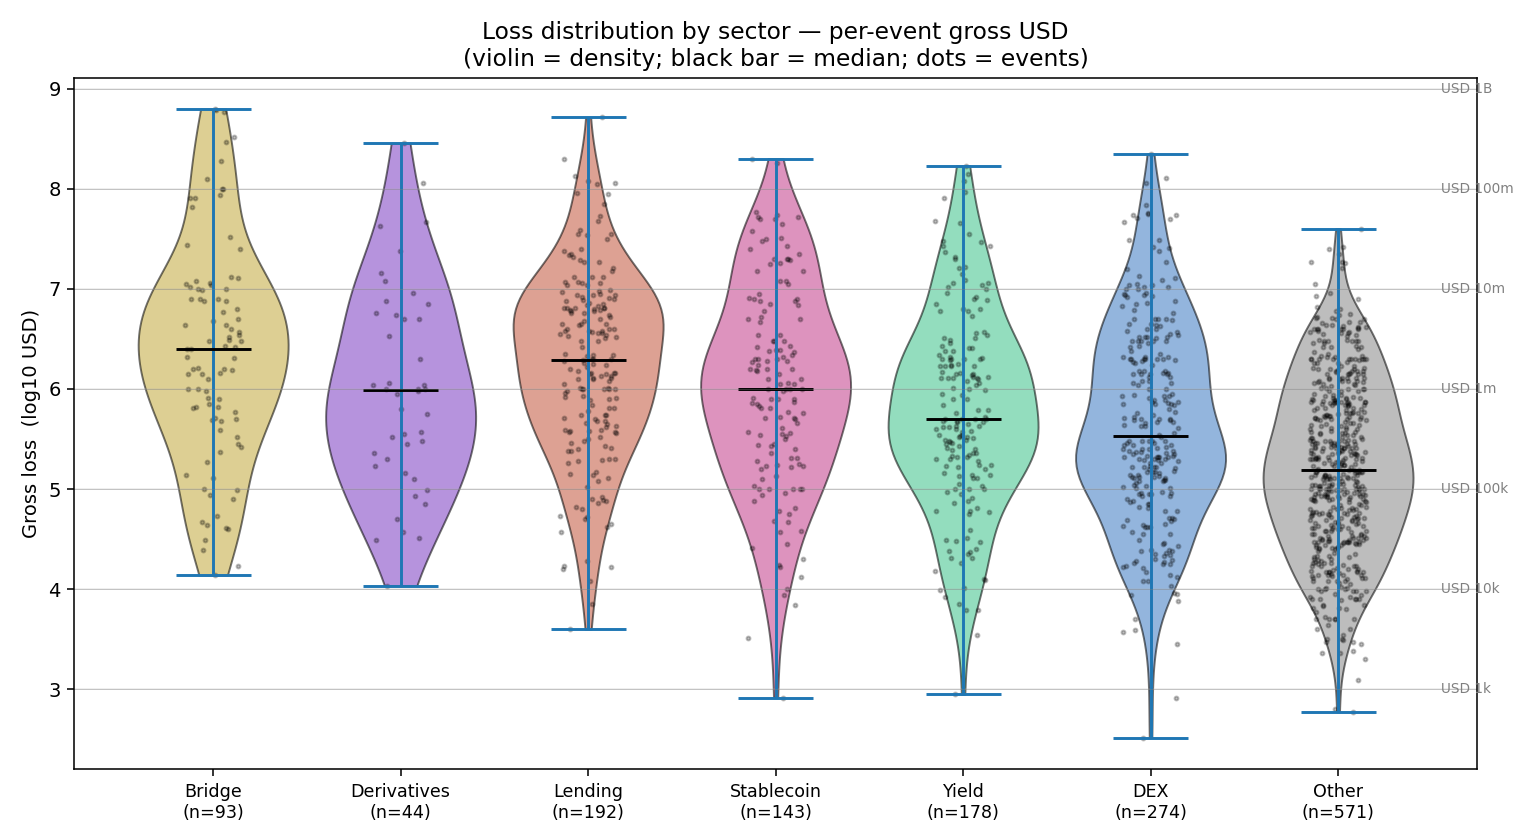
\includegraphics[width=\linewidth]{figures/r0b_loss_distribution_by_sector.png}
\caption{Loss distribution by DeFi sector ($n=1{,}495$). Violin
shape encodes density, black bar is the median, dots are
individual events. Sample-size labels on the $x$-axis. The shape
of the distribution differs materially across sectors: Bridge has
a high median and a thin extreme tail anchored on a small number
of mega-events; Lending and Stablecoin show heavier tails with
materially larger right-side mass; Yield and DEX have lower
medians but extreme outliers; Other is body-dominated. These
differences foreshadow the per-sector EVT fits in
\S\ref{sec:severity}.}
\label{fig:lossdist}
\end{figure}

The qualitative features apparent in Figure~\ref{fig:lossdist}
matter for everything that follows. \textbf{Bridge} carries by far
the highest \emph{median} event loss (USD~2.5~m) and the largest
extreme value (Ronin, USD~624~m): bridges hold pooled cross-chain
collateral whose unit value is structurally large, so even
mid-sized events scale into the millions. \textbf{Lending} sits
second on median (USD~1.9~m) with a long upper tail anchored on
Vires Finance (USD~515~m), Euler V1 (USD~197~m), CREAM
(USD~130~m), and BonqDAO (USD~120~m). \textbf{Stablecoin} (median
USD~1.1~m) and \textbf{Derivatives} (median USD~1.0~m) carry
mid-sized typical events with a sparse handful of large outliers.
\textbf{DEX} (median USD~0.35~m) and \textbf{Yield} (median
USD~0.50~m) carry many smaller events with extreme outliers
(Cetus CLMM USD~223~m on DEX; YFValue USD~170~m on Yield).
\textbf{Other} (median USD~0.20~m) is the long tail of small,
low-cap events that contributes 38\% of count but only 5\% of
USD aggregate. Aggregate USD by sector, in descending order:
Bridge USD~3.60~B ($n=93$), Lending USD~2.41~B ($n=192$), DEX
USD~1.51~B ($n=274$), Stablecoin USD~1.34~B ($n=143$), Yield
USD~1.20~B ($n=178$), Derivatives USD~0.60~B ($n=44$), Other
USD~0.59~B ($n=571$).

\subsection{Sector $\times$ event-type cross-tabulation}\label{sec:cross-tab}

Sector (\S\ref{sec:sector}) and Basel III Level-1 event type
(\S\ref{sec:riskcat}) are conceptually orthogonal: the former
captures the \emph{economic function} of the protocol affected, the
latter the \emph{operational mechanism} of the loss event. Crossing
the two reveals which sector~$\times$~event-type pairs dominate
event counts and USD losses. Table~\ref{tab:sector-basel-n}
(counts) and Table~\ref{tab:sector-basel-usd} (USD~m) give the full
cross-tabulation.

\begin{table}[h]
\centering
\small
\begin{tabular}{l r r r r r r}
\toprule
Sector $\backslash$ Event type & EF & IF & CPBP & EDPM & BDSF & \textbf{Total} \\
\midrule
Stablecoin   &  78 &  27 &  35 &  2 &  1 & \textbf{143}   \\
Lending      &  86 &  15 &  78 & 11 &  2 & \textbf{192}   \\
DEX          & 153 &  56 &  61 &  1 &  3 & \textbf{274}   \\
Yield        &  71 &  56 &  42 &  5 &  4 & \textbf{178}   \\
Derivatives  &  27 &   4 &  12 &  0 &  1 & \textbf{44}    \\
Bridge       &  72 &  11 &   7 &  2 &  1 & \textbf{93}    \\
Other        & 342 & 156 &  59 &  5 &  9 & \textbf{571}   \\
\midrule
\textbf{Total}  & \textbf{829} & \textbf{325} & \textbf{294} & \textbf{26} & \textbf{21} & \textbf{1{,}495} \\
\bottomrule
\end{tabular}
\caption{Number of operational-risk events by sector $\times$
Basel~III Level-1 event-type category. EPWS and DPA columns
omitted (both zero by construction in DeFi). EF (external attacks
on smart-contract code, keys, and auxiliary infrastructure)
dominates every sector; CPBP (economic-design / oracle / governance
events) is the secondary mechanism in financial-primitive sectors
(Lending, Stablecoin, DEX, Yield) but largely absent from Bridge.}
\label{tab:sector-basel-n}
\end{table}

\begin{table}[h]
\centering
\small
\begin{tabular}{l r r r r r r}
\toprule
Sector $\backslash$ Event type & EF & IF & CPBP & EDPM & BDSF & \textbf{Total} \\
\midrule
Stablecoin   &    723 &  163 &   365 &  54 &   2 & \textbf{1{,}305} \\
Lending      &    776 &  562 & 1{,}040 &  12 &  16 & \textbf{2{,}405} \\
DEX          & 1{,}114 &  213 &   151 &   0 &   0 & \textbf{1{,}478} \\
Yield        &    759 &   84 &   338 &  17 &   2 & \textbf{1{,}200} \\
Derivatives  &    171 &    2 &   143 &   0 & 285 & \textbf{601}    \\
Bridge       & 3{,}412 &   56 &   108 &  11 &  12 & \textbf{3{,}598} \\
Other        &    440 &   98 &    15 &   5 &  35 & \textbf{592}    \\
\midrule
\textbf{Total}  & \textbf{7{,}394} & \textbf{1{,}177} & \textbf{2{,}159} & \textbf{98} & \textbf{352} & \textbf{11{,}180} \\
\bottomrule
\end{tabular}
\caption{Aggregate gross loss (USD~m) by sector $\times$ Basel~III
Level-1 event-type category. Cells reveal three sharply different
loss-generation regimes: Bridge USD aggregate is $\sim$95\% EF
(Poly, Ronin, BSC Token Hub, Wormhole, Nomad, Cetus are all
external-attack events on bridge logic); Lending USD aggregate is
dominated by CPBP (USD~1.04~B in economic-design / oracle /
undercollateralised-borrow events) over EF (USD~0.78~B);
Stablecoin and Yield USD aggregates are roughly split
EF/CPBP/IF, reflecting the mix of code attacks, mechanism attacks,
and insider rugpulls in those sectors. The single largest USD
cell in the table is Bridge $\times$ EF (USD~3.41~B = 31\% of
aggregate loss).}
\label{tab:sector-basel-usd}
\end{table}

Three patterns emerge that anticipate the later formal results.

\textbf{Bridge losses are almost a single-mechanism story.}
72 of 93 Bridge events (77\%) and USD~3.41~B of USD~3.60~B in Bridge
losses (95\%) are EF --- external smart-contract / key attacks on
cross-chain components. The Bridge severity tail in the per-sector
EVT fits of \S\ref{sec:severity} is, mechanically, the EF tail.
What makes Bridge structurally heavier-loss is not the mix of
mechanisms but the collateral value locked in the smart contracts
that are subject to operational-risk events.

\textbf{Lending loss USD is a CPBP story, not an EF story.}
Lending is the only sector in the dataset where CPBP USD
(USD~1.04~B) exceeds EF USD (USD~0.78~B). The 78 CPBP Lending events
include Euler V1 (USD~197~m), BonqDAO (USD~120~m), Mango Markets
oracle manipulation, and the long sequence of flashloan-oracle
attacks against money-markets-with-thin-oracle on long-tail
collateral. This is a mechanism-attack profile that the
external-attacker EF rubric does not capture cleanly: the protocol
code did exactly what it was specified to do, but the economic-
design assumption (oracle accuracy, collateral liquidity, governance
honesty) failed under adversarial conditions. The implication for
later sections is that a pooled Lending tail-shape fit is averaging
two materially different mechanisms.

\textbf{IF is concentrated in Yield and Other.}
Of 325 IF events, 212 (65\%) are in Yield and Other, the two sector
buckets that contain the bulk of low-cap rugpullable protocols.
By USD, however, IF is anchored by a handful of mid-cap Lending
insider events (Vires Finance USD~515~m, plus several CeFi-style
lending desks) whose USD impact disproportionately outweighs their
count. The asymmetry says that the IF \emph{rate} per dollar of
TVL is concentrated in the long-tail rugpullable space, while
the IF \emph{tail loss} is concentrated where mid-cap Lending
protocols ran without independent custody of user assets.

\subsection{Events over time}\label{sec:timeplot}

The temporal distribution of events is the third descriptive cut
we need before fitting any model.
Figure~\ref{fig:events-scatter} plots every event in the dataset
as a log-scale loss-vs-date scatter, colour-coded by Basel~III
Level-1 event type.

\begin{figure}[h]
\centering
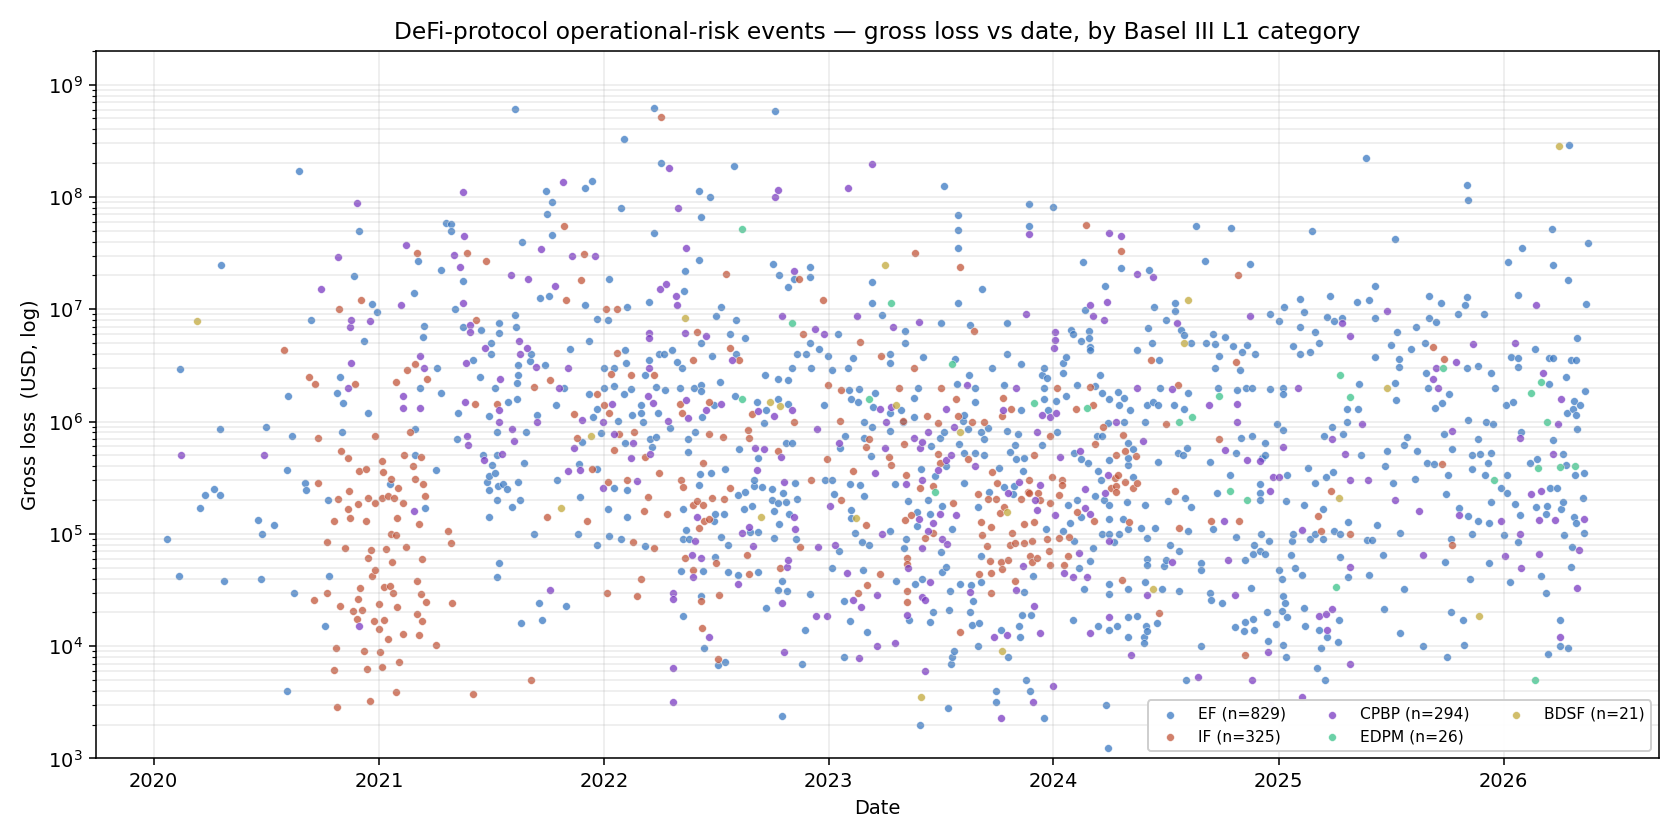
\includegraphics[width=\linewidth]{figures/r0_events_scatter.png}
\caption{Every operational-risk event in the dataset, gross loss
(USD, log) vs date, by Basel~III Level-1 event type.}
\label{fig:events-scatter}
\end{figure}

A clearer view of \emph{intensity} comes from rolling 90-day event
counts per group. Figure~\ref{fig:rolling} plots the rolling event
intensity per sector (left panel) and per Basel~III Level-1 event
type (right panel), reported as events per 30~days (a 90-day
window divided by 3) so that the units are directly comparable to
monthly rates.

\begin{figure}[h]
\centering
\begin{subfigure}[t]{0.49\linewidth}
\centering
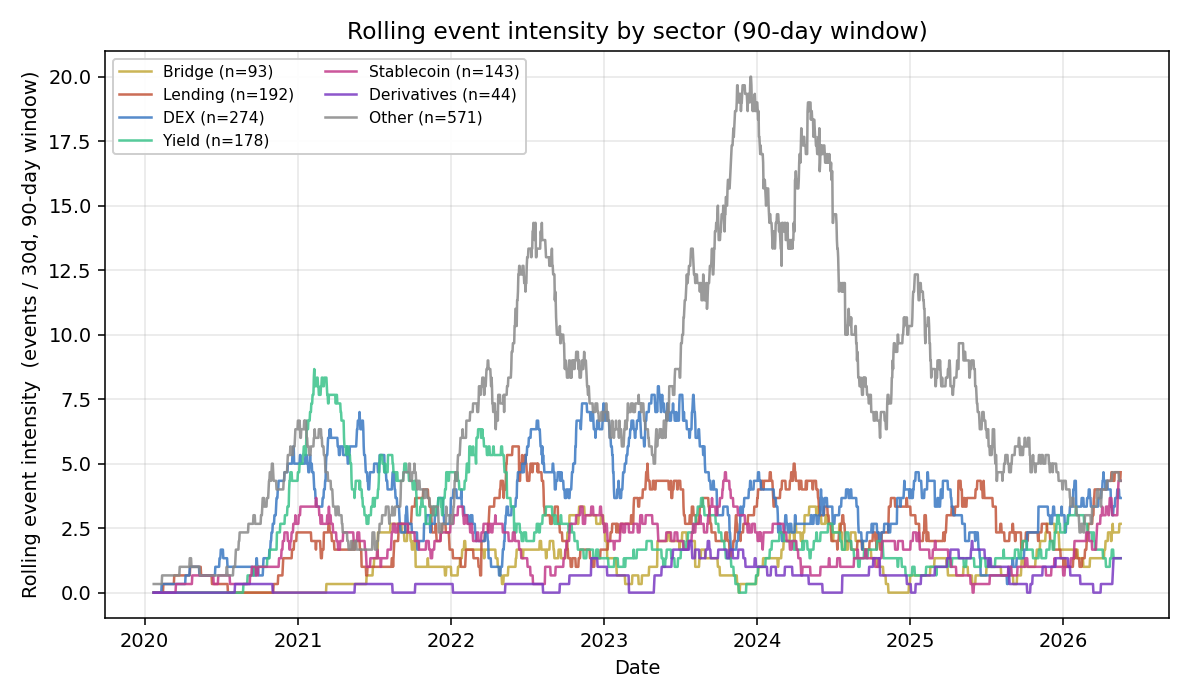
\includegraphics[width=\linewidth]{figures/r0c_rolling_intensity_sector.png}
\caption{By sector.}
\label{fig:rolling-sector}
\end{subfigure}
\hfill
\begin{subfigure}[t]{0.49\linewidth}
\centering
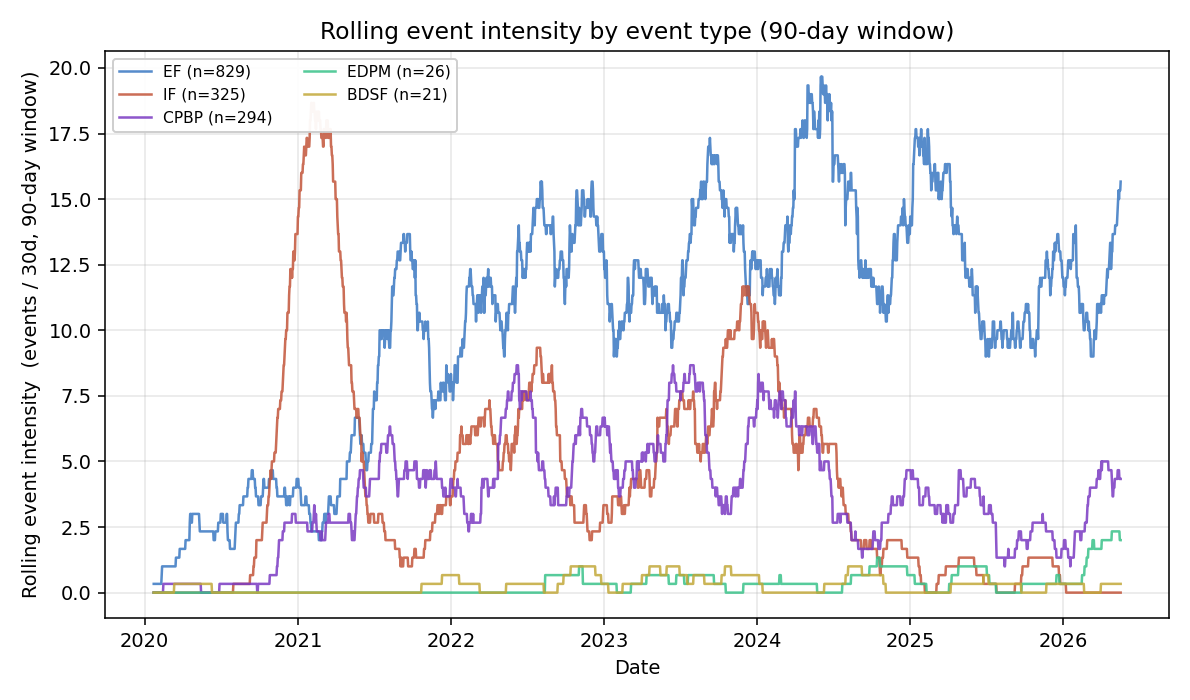
\includegraphics[width=\linewidth]{figures/r0d_rolling_intensity_basel.png}
\caption{By Basel~III Level-1 event type.}
\label{fig:rolling-basel}
\end{subfigure}
\caption{Rolling 90-day event intensity (events per 30-day
equivalent). \emph{Left:} the Other bucket carries most of the
post-2022 growth in count (long-tail rugpulls / flashloan attacks
on low-cap protocols); Lending, Bridge, DEX, and Yield each
contribute 1--5 events / 30d in the stationary regime.
\emph{Right:} the 2021 IF spike is the rugpull / exit-scam wave on
the low-cap yield-aggregator and farm-token bucket; EF dominates
from 2022 onward as the cross-chain bridge attacks and the
flashloan-oracle exploit toolchain mature; CPBP rises through
2023--2024 as oracle-manipulation patterns are reused across the
expanding lending and stablecoin substrate. EDPM and BDSF remain
low-rate categories throughout.}
\label{fig:rolling}
\end{figure}

The combined picture from the scatter and the two rolling-intensity
panels is that the relative composition of sectors and event-type
categories rotates materially over time --- features that the
formal models of \S\ref{sec:severity}--\S\ref{sec:lda} will absorb
into the per-sector frequency parameters.

\subsection{Methodological implication: fit per sector}\label{sec:explore-patterns}

The three descriptive cuts above motivate a methodological choice
that shapes the rest of the paper: \textbf{aggregating across
sectors does not make sense.} The sector~$\times$~event-type
cross-tabulation of \S\ref{sec:cross-tab} shows that the dominant
operational mechanism varies materially by sector: Bridge is a
near-pure EF~/~access-control story (95\% EF by USD), Lending is
a CPBP mechanism story (43\% CPBP by USD), Yield and Other carry
most of the IF~/~rugpull \emph{rate}, and Stablecoin shows a
mixed EF~/~CPBP~/~EDPM profile reflecting the diversity of
underlying designs. A pooled severity tail would average these
distinct loss-generation processes, mask the variation in the
tail-shape parameter $\xi$ across sectors, and produce a
sample-mean estimator that is dominated by whichever sector
happens to contain the largest historical event in the data
window. The per-sector loss distribution in
Figure~\ref{fig:lossdist} confirms this visually: the violin
shapes are materially different across sectors, particularly in
the upper-tail mass. We therefore fit POT-GPD severity and the
LDA capital-requirement Monte Carlo \emph{per sector}, with
pooled-DeFi numbers reported alongside as a reference rather than
as the operationally meaningful capital figure.
Table~\ref{tab:top15} lists the fifteen largest events in the
dataset: six are Bridge (Ronin, Poly, Binance Bridge,
Portal/Wormhole, Kelp, Nomad), three are Lending, the remaining
six split across Stablecoin, Yield, DEX, and Derivatives --- a
sector composition that no single-sector fit could reproduce and
no pooled fit would faithfully decompose.

\begin{table}[h]
\centering
\small
\begin{tabular}{l l r l l}
\toprule
Date & Event & USD~m & Sector & Event type \\
\midrule
2022-03-23 & Ronin Bridge          & 624 & Bridge      & EF   \\
2021-08-10 & Poly Network          & 611 & Bridge      & EF   \\
2022-10-06 & Binance Bridge        & 570 & Bridge      & EF   \\
2022-04-03 & Vires Finance         & 515 & Lending     & IF   \\
2022-02-02 & Portal (Wormhole)     & 326 & Bridge      & EF   \\
2026-04-18 & Kelp (rsETH)          & 293 & Bridge      & EF   \\
2026-04-01 & Drift Trade           & 285 & Derivatives & BDSF \\
2025-05-22 & Cetus CLMM            & 223 & DEX         & EF   \\
2022-04-04 & Neutrino USD          & 200 & Stablecoin  & EF   \\
2023-03-13 & Euler V1              & 197 & Lending     & CPBP \\
2022-08-01 & Nomad                 & 190 & Bridge      & EF   \\
2022-04-17 & Beanstalk             & 181 & Stablecoin  & CPBP \\
2020-08-24 & YFValue               & 170 & Yield       & EF   \\
2021-09-29 & Compound V2           & 147 & Lending     & EF   \\
2021-12-13 & Vulcan Forged         & 140 & Yield       & EF   \\
\bottomrule
\end{tabular}
\caption{The fifteen largest operational-risk events in the
dataset, by gross USD loss. Six of fifteen are Bridge events;
three Lending; the remaining six split across Stablecoin, Yield,
DEX, and Derivatives. Eleven of fifteen are EF (external attack
on smart-contract code, keys, or auxiliary infrastructure), two
CPBP (economic-design event), one IF (insider exit), one BDSF
(chain-level / business-disruption).}
\label{tab:top15}
\end{table}

% ===========================================================================
\section{Severity tail: how heavy is heavy?}\label{sec:severity}
% ===========================================================================

We treat individual event gross losses as iid draws from a severity
distribution $F_X$ and ask how heavy the upper tail is, by every
diagnostic and parametric fit in the EVT toolkit.

\subsection{Diagnostics}

\textbf{Log-log CCDF.} Figure~\ref{fig:loglogccdf} plots the empirical
complementary cumulative distribution $\bar F(x) = \Pr(X \geq x)$ on
log-log axes for each major sector with the Clauset MLE power-law fit
overlaid. Above approximately USD 5~m the DeFi curve is
approximately a straight line over three orders of magnitude --- a
necessary signature of a Pareto-type tail.

\begin{figure}[h]
\centering
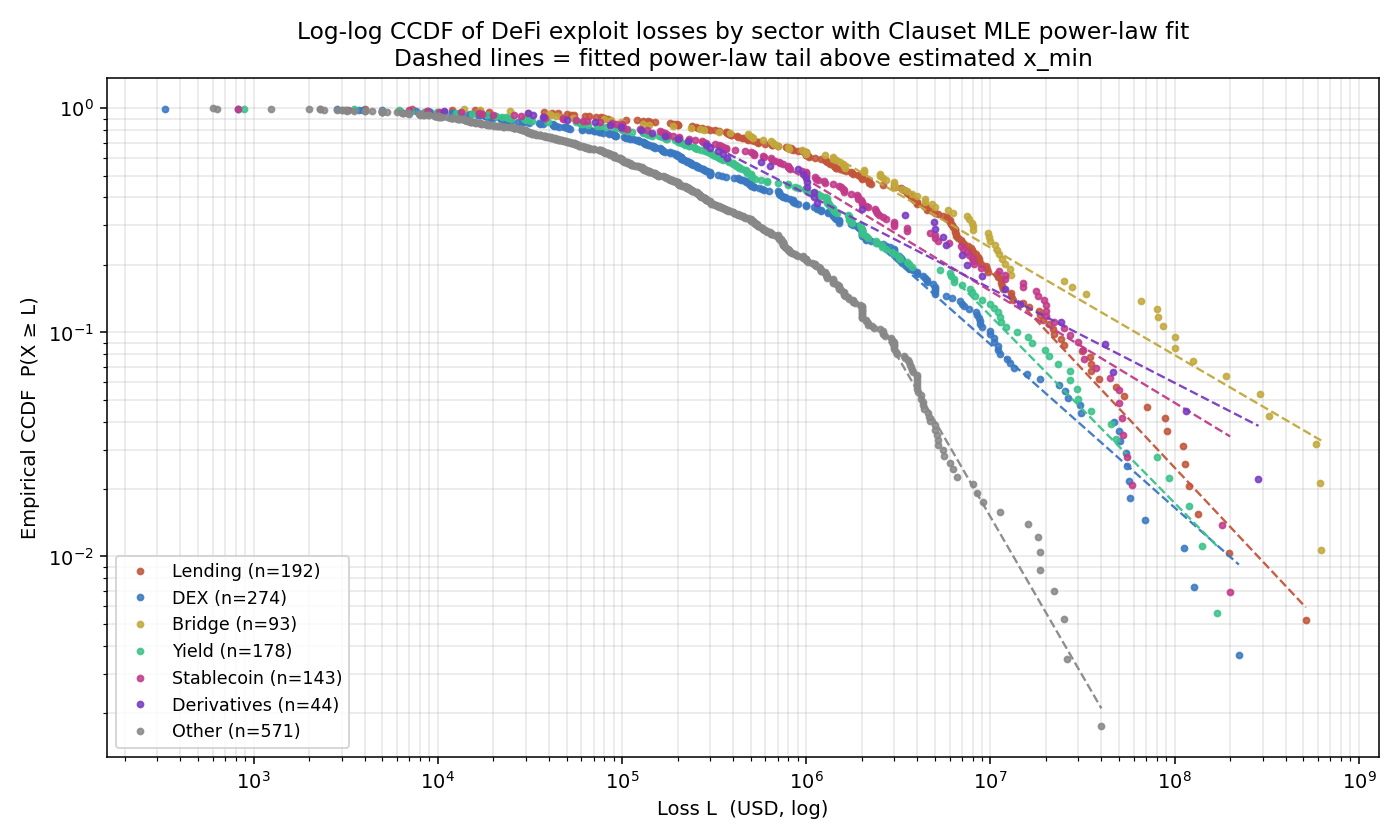
\includegraphics[width=0.85\linewidth]{r3_loglog_ccdf.png}
\caption{Empirical log-log CCDF $\Pr(X \geq L)$ by sector, with
Clauset MLE power-law fits overlaid (dashed lines) above the
fitted $x_{\min}$. Approximately straight-line behaviour over three
orders of magnitude in the DeFi tail.}
\label{fig:loglogccdf}
\end{figure}

\textbf{Mean excess.} For a generalized-Pareto excess distribution the
mean excess function
$e(u) = \E[X-u \mid X>u]$
is linear in $u$ with positive slope $\xi/(1-\xi)$.
Figure~\ref{fig:meanexcess} plots $e(u)$ for each sector on log-log
axes: the DeFi curve is monotonically increasing and near-linear
in $\log u$ across two decades, consistent with $\xi>0$, i.e.\ the
Fréchet (Pareto-type) max-domain of attraction.

\textbf{Hill estimator.} For order statistics
$X_{(1)} \geq X_{(2)} \geq \dots \geq X_{(n)}$, the Hill estimator
based on the top $k+1$ values is
\begin{equation}\label{eq:hill}
\hat\xi_H(k) \;=\; \frac{1}{k}\sum_{i=1}^{k}\ln X_{(i)} \;-\; \ln X_{(k+1)}.
\end{equation}
Figure~\ref{fig:hill} plots $\hat\xi_H(k)$ over $k\in[5, n/2]$. The
DeFi Hill curve sits in the band $[0.9, 1.2]$ across a wide
stable range of $k\in[50, 400]$, plateau-region evidence for a tail
index right at the infinite-mean threshold $\xi \geq 1$.

\begin{figure}[h]
\centering
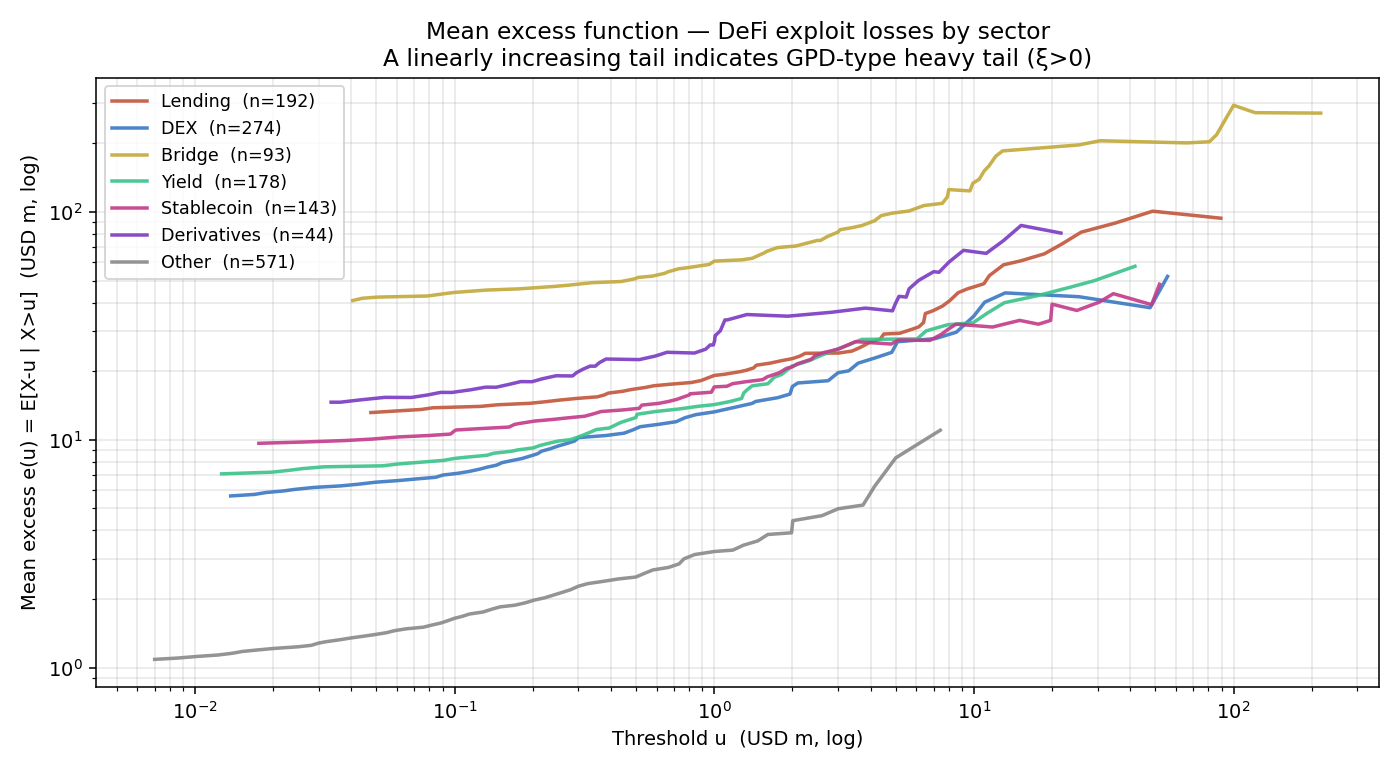
\includegraphics[width=0.85\linewidth]{r1_mean_excess.png}
\caption{Mean excess function $e(u) = \E[X-u \mid X>u]$ by sector
(log-log axes). Approximately linear $e(u)$ in $\log u$ over two decades
is consistent with a Pareto-type (Fréchet) tail. Bridge is offset
vertically due to a few mega-events at the top of the distribution.}
\label{fig:meanexcess}
\end{figure}

\begin{figure}[h]
\centering
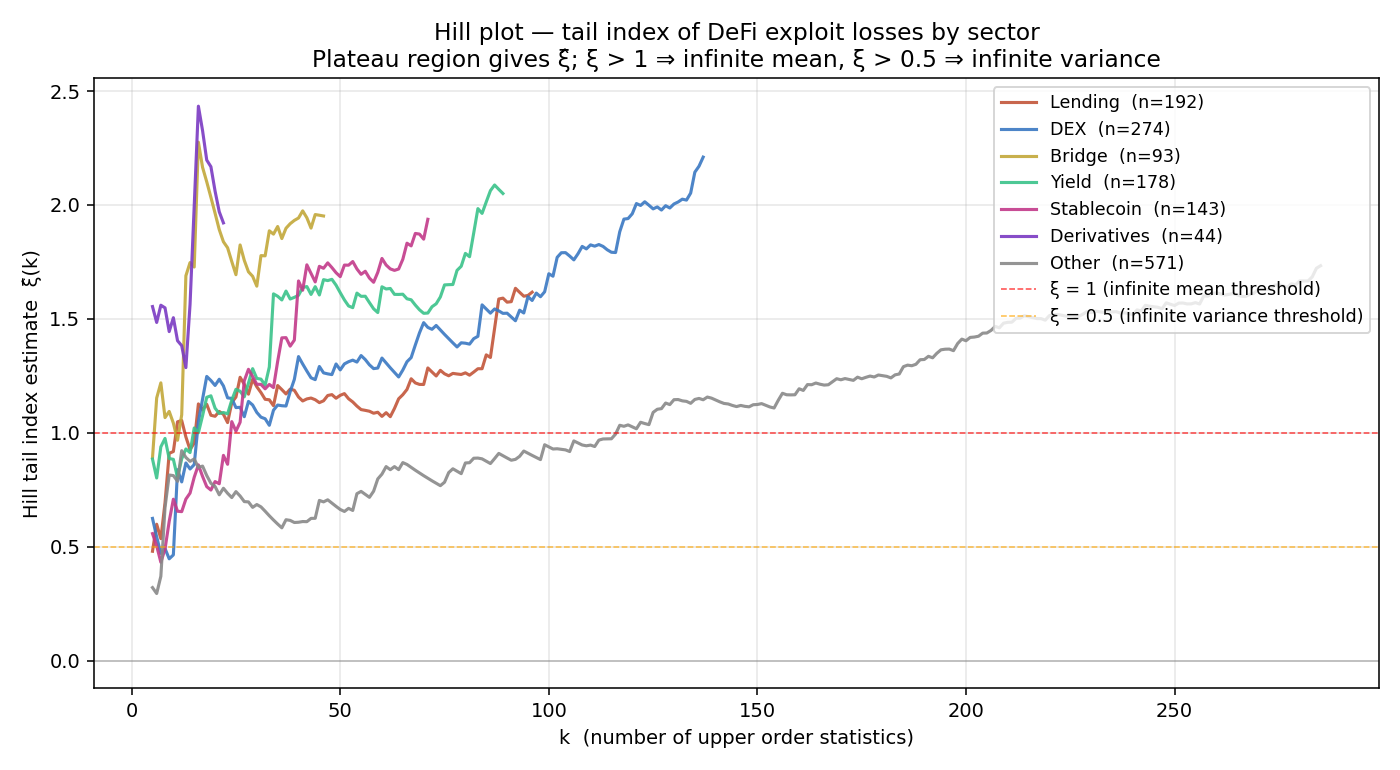
\includegraphics[width=0.85\linewidth]{r2_hill_plot.png}
\caption{Hill plot $\hat\xi_H(k)$ by sector. Pooled-DeFi (black) sits
in $[0.9, 1.2]$ across a stable plateau in $k$, evidence for a tail
index right at the infinite-mean boundary. Dashed lines: $\xi=0.5$
(infinite variance threshold) and $\xi=1$ (infinite mean threshold).}
\label{fig:hill}
\end{figure}

\subsection{POT-GPD maximum likelihood}\label{sec:potgpd}

For a threshold $u$ and excesses $Y_i = X_i - u \mid X_i>u$, the
generalized-Pareto density is
\begin{equation}
g_{\xi,\beta}(y)
  \;=\; \frac{1}{\beta}\,\Bigl(1 + \xi\,\frac{y}{\beta}\Bigr)^{-(1/\xi + 1)},
  \qquad y>0,\ \beta>0,\ \xi\in\mathbb{R}.
\end{equation}
We fit $(\xi,\beta)$ by maximum likelihood with multi-start
Nelder--Mead, choosing the threshold quantile $q$ automatically
per sector to maintain at least 20--30 exceedances (the standard
POT-GPD compromise between bias from a too-low threshold and
variance from a too-high one).

\textbf{Per-sector POT-GPD fits.} Table~\ref{tab:per-sector-pot}
summarises the headline POT-GPD fit per sector. Threshold quantile
is chosen automatically to maintain at least 20--30 exceedances where
sample size allows.

\begin{table}[h]
\centering
\small
\begin{tabular}{lrrrrr}
\toprule
Sector  & $n$ & $q^*$ & $u^*$ (USD m) & $\hat\xi$ & $\hat\beta$ (USD m) \\
\midrule
Stablecoin             &     143 & 0.80 &  8.1 & +0.298 &  22.2 \\
\textbf{Lending}       &     192 & 0.80 &  8.9 & \textbf{+0.925} &  13.1 \\
DEX                    &     274 & 0.85 &  5.0 & +0.623 &  12.7 \\
Yield                  &     178 & 0.80 &  3.6 & +0.589 &  13.2 \\
Derivatives            &      44 & 0.70 &  5.0 & +1.576 &   4.7 \\
Bridge                 &      93 & 0.80 & 11.8 & +0.599 &  86.0 \\
Other                  &     571 & 0.85 &  1.6 & +0.505 &   2.0 \\
\bottomrule
\end{tabular}
\caption{POT-GPD fits per sector. \textbf{Lending} sits just below
the infinite-mean boundary ($\hat\xi=0.93$); DEX, Bridge, and Yield
fit moderately-heavy $\hat\xi\in[0.59, 0.62]$; Stablecoin fits a
markedly lighter $\hat\xi=0.30$. \textbf{Derivatives} ($n=44$,
$\hat\xi=1.58$) is sample-size-limited and the high shape estimate
is dominated by a small number of nine-figure events (Drift Trade
USD~285~m, GMX V1, FTX validator etc.); it should not be taken as
a credible per-sector tail-index and is flagged accordingly in the
LDA below. The paper does not produce a pooled-DeFi POT-GPD fit:
all severity work is per sector.}
\label{tab:per-sector-pot}
\end{table}

Three observations on the per-sector results.

\emph{First}, \textbf{Lending fits right at the infinite-mean
boundary} ($\hat\xi=0.93$, $n=192$, q=0.80, $u=$~USD~8.9~m).
DeFi-Lending exposures are therefore close to not insurable on
standard premium principles: the sample mean of historical losses
is a statistically unstable estimator that depends arbitrarily
strongly on the next single large event (Vires Finance USD~515~m,
Euler V1 USD~197~m, Compound V2 USD~147~m, CREAM Lending
USD~130~m).

\emph{Second}, \textbf{Stablecoin, DEX, Yield, and Bridge fit in
the moderate-to-heavy OpRisk range} ($\hat\xi \in [0.30, 0.62]$),
within the Moscadelli (2004) Basel-II banking-OpRisk band of
$[0.85, 1.39]$ on the lighter side. These tails are insurable on
standard premium principles, and the LDA capital figures below are
the corresponding bank-Pillar-II-equivalent numbers.

\emph{Third}, \textbf{Bridge is the largest sector by aggregate loss
(USD~3.60~B) but its formal EVT fit is sample-size-limited}. With
$n=93$ records and a small handful of nine-figure mega-events
(Ronin USD~624~m, Poly Network USD~611~m, Binance Bridge
USD~570~m, Wormhole USD~326~m, Portal USD~326~m, Nomad USD~190~m,
Multichain USD~126~m, Kelp USD~293~m, Harmony USD~100~m, Orbit
USD~82~m), the mean-excess function sits an order of magnitude
above any other sector at all thresholds; the Bridge tail-shape
estimate should be read with caution.

\subsection{POT-GPD goodness-of-fit}

Figure~\ref{fig:gpdqq} is the QQ plot of empirical excesses against
the fitted-GPD quantiles for Lending --- the headline-capital
sector --- at the 80th-percentile threshold. The fit is essentially
a straight line across the empirical tail, with mild over-shoot at
the very top of the distribution: the largest excesses (Vires
Finance, Euler V1) sit slightly below the fitted line, i.e.\ the
data are very slightly \emph{heavier} than the GPD fit at $q=0.80$.

\begin{figure}[h]
\centering
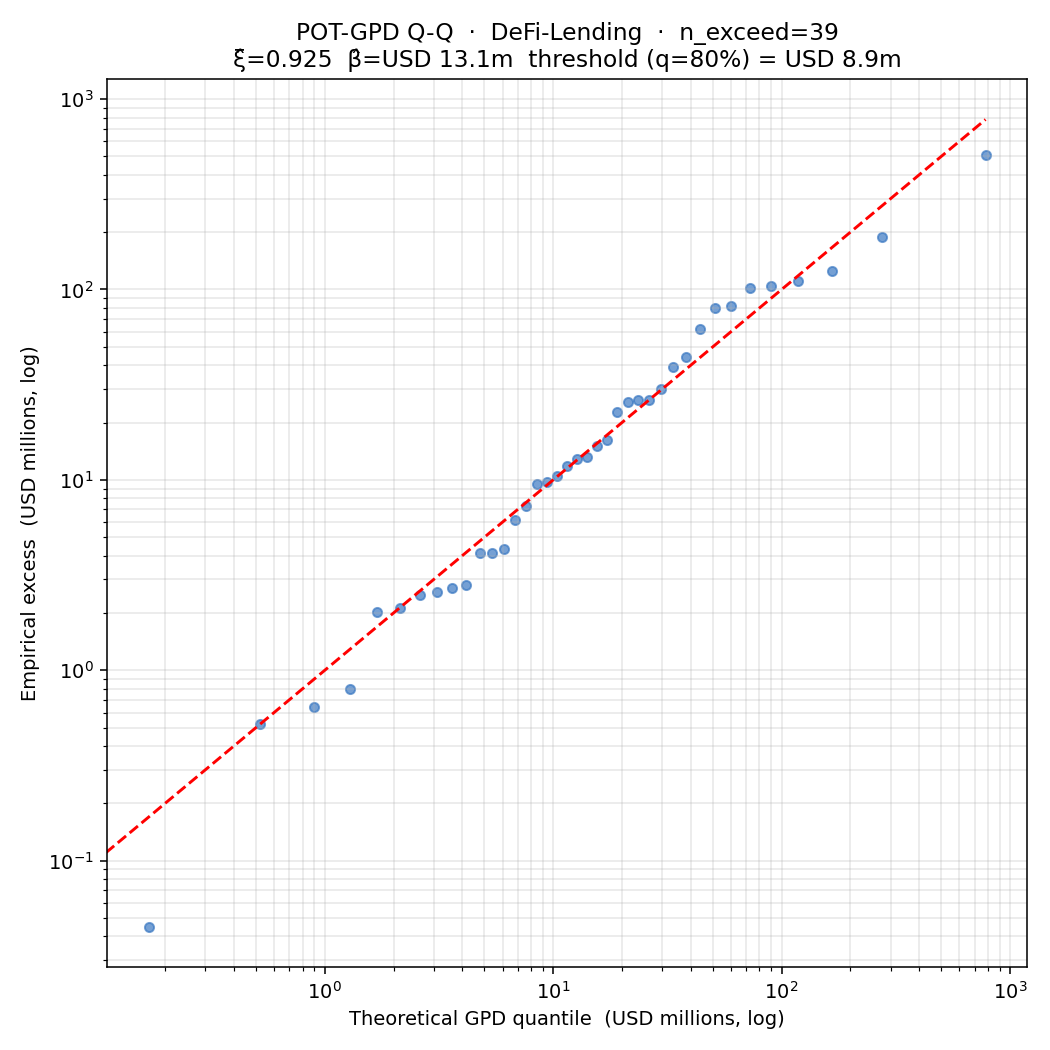
\includegraphics[width=0.55\linewidth]{r4_gpd_qq_lending.png}
\caption{POT-GPD QQ diagnostic for the DeFi Lending sector at the
80th-percentile threshold ($u=$~USD~8.9~m). Empirical and
theoretical quantiles align across the tail.}
\label{fig:gpdqq}
\end{figure}

\subsection{Power-law fit and lognormal benchmark}

Following \citet{Clauset2009}, we fit a continuous power-law density
on $X \geq x_{\min}$ by
\begin{equation}
\hat\alpha
  \;=\;
  1 + n \!\left/\sum_{i:x_i\geq x_{\min}}\!\!\!\log\frac{x_i}{x_{\min}}\right.,
  \qquad
  \hat x_{\min}
  \;=\;
  \arg\min_{x_{\min}}\,D_{\text{KS}}\!\left(\hat F, F_{\hat\alpha}\right),
\end{equation}
where $D_{\text{KS}}$ is the Kolmogorov-Smirnov distance between the
empirical CDF and the fitted-Pareto CDF, both evaluated on
$x \geq x_{\min}$. For DeFi we obtain $\hat\alpha=1.75$,
$\hat x_{\min}\!\approx\!$ USD~4~m, with KS distance below~0.05 over
$n_{\text{tail}}\sim 290$. The conversion identity
$\xi = 1/(\alpha-1)$ gives $\xi\!\approx\!1.33$, broadly consistent
with the Hill plateau and slightly heavier than the POT-GPD fit at
$q=0.85$.

A Vuong-style log-likelihood comparison between the power-law fit and
a lognormal restricted to the same tail gives a near-tied result in
every sector ($|\Delta \ell| \leq 3$). This is the standard
\citet{Clauset2009} finding for heavy-tailed empirical data:
distinguishing pure-power-law from lognormal on the tail alone is
statistically difficult at our sample size, but \emph{both} alternatives
are firmly in the subexponential class. What follows in this paper
does not require us to distinguish the two; the GPD already
parameterises both as limiting cases.

\subsection{Cross-field benchmark of tail indices}

Figure~\ref{fig:tailbench} places the DeFi $\hat\xi$ estimates from
the sector breakdown on the same horizontal scale as published
ranges for other loss-generating processes. The cross-field summary
is:

\begin{table}[h]
\centering
\small
\begin{tabular}{lr}
\toprule
Process & $\xi$ range \\
\midrule
Equity daily log-returns (S\&P) & 0.20--0.40 \\
Hurricane / NatCat insured losses & 0.50--1.00 \\
Major-earthquake economic losses & 0.60--1.10 \\
Cyber-breach losses (Eling \& Wirfs 2019) & 0.70--1.10 \\
Banking operational risk (Moscadelli 2004, BIS QIS) & 0.85--1.20 \\
\textbf{DeFi-Lending (this paper)} & \textbf{0.93} \\
\textbf{DeFi-DEX / Yield / Bridge (this paper)} & \textbf{0.59--0.62} \\
\textbf{DeFi-Stablecoin (this paper)} & \textbf{0.30} \\
\bottomrule
\end{tabular}
\caption{Tail-index $\xi$ ranges across loss-generating processes.
DeFi-Lending fits just below the infinite-mean boundary and is
statistically indistinguishable from \citet{Moscadelli2004}'s
canonical Basel~II banking operational-risk range; DEX, Yield,
and Bridge fit in the moderate-heavy OpRisk range; Stablecoin
fits markedly lighter. Derivatives ($\hat\xi=1.58$, $n=44$) is
sample-size-limited and is not benchmarked here.}
\end{table}

\begin{figure}[h]
\centering
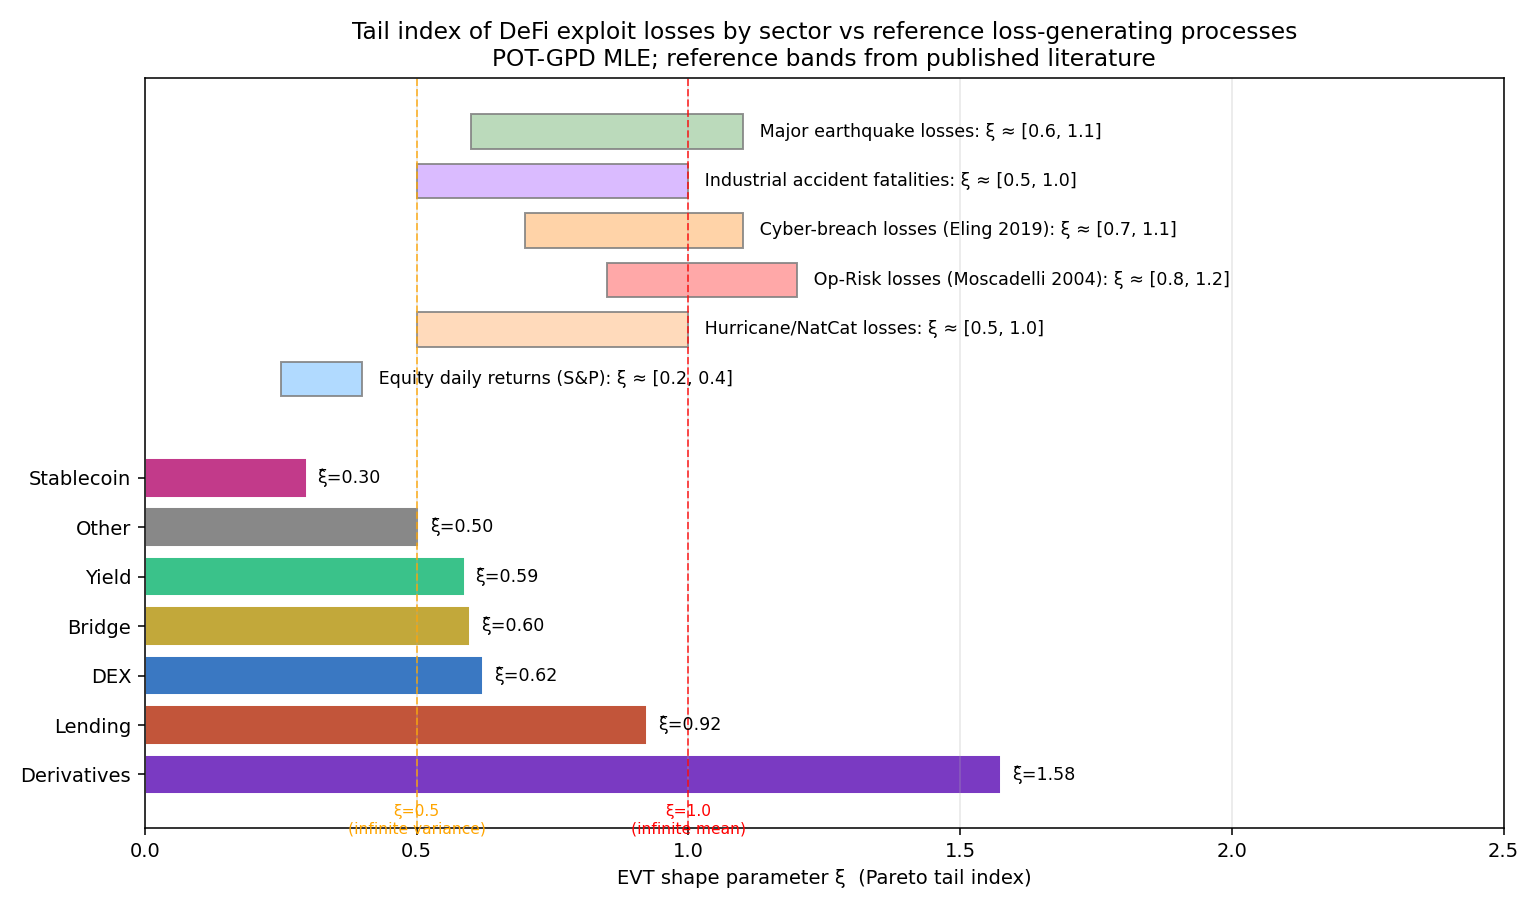
\includegraphics[width=0.85\linewidth]{r5_tail_index_benchmarks.png}
\caption{DeFi tail indices by \textbf{sector} vs reference loss-
generating processes. Fitted by POT-GPD; reference bands from
published literature.}
\label{fig:tailbench}
\end{figure}

% ===========================================================================
\section{Frequency: per-sector event rates and cross-sector over-dispersion}\label{sec:freq}
% ===========================================================================

The LDA in \S\ref{sec:lda} requires a per-sector annual event
rate. The rate enters as the Poisson intensity of the compound
distribution; the over-dispersion question --- whether the
monthly arrival process is Poisson or negative-binomial --- is a
modelling decision that matters at the aggregate cross-sector
level, where the LDA simulator generates correlated event years.

\subsection{Per-sector annual rates}\label{sec:per-sector-lambda}

We compute the per-sector annual rate as
$\hat\lambda_s = n_s / T$ where $T = 6.3$ years is the analysis
window length and $n_s$ is the per-sector event count from
Table~\ref{tab:sector-basel-n}. The resulting per-sector rates
are: Lending $30.4$/yr, DEX $43.4$/yr, Yield $28.2$/yr, Bridge
$14.7$/yr, Stablecoin $22.7$/yr, Derivatives $7.0$/yr, Other
$90.6$/yr. These rates enter the per-sector LDA Monte Carlo
directly.

\subsection{Cross-sector monthly counts and over-dispersion}

The per-sector LDA does not require a pooled frequency
distribution, but the cross-sector monthly count series is
informative for diagnosing whether the event arrival process
satisfies the Poisson assumption that underlies the LDA Monte
Carlo. The 76 monthly counts
have mean $\bar X = 19.9$, variance $s^2 = 78.0$, dispersion
index $D = s^2/\bar X = 3.92$. The Cameron--Trivedi
over-dispersion test rejects equidispersion overwhelmingly
($z \approx 18$, $p \approx 0$). A negative-binomial
$\NB(\mu,\alpha)$ fit gives
$(\hat\mu, \hat\alpha) \approx (19.9, 0.21)$ and a likelihood-ratio
test against the nested Poisson rejects at $p \approx 0$ (LR
$\approx 134$). The dispersion is partly driven by the 2020--2023
ramp and partly by genuine within-month clustering across sectors;
on the 2021--2026 stationary subset the residual over-dispersion
remains.

Figure~\ref{fig:monthly} shows the monthly time series and the
count-distribution histogram with both Poisson and negative-binomial
fitted PMFs. The NB fit captures the right tail of busy months that
Poisson under-counts.

\begin{figure}[h]
\centering
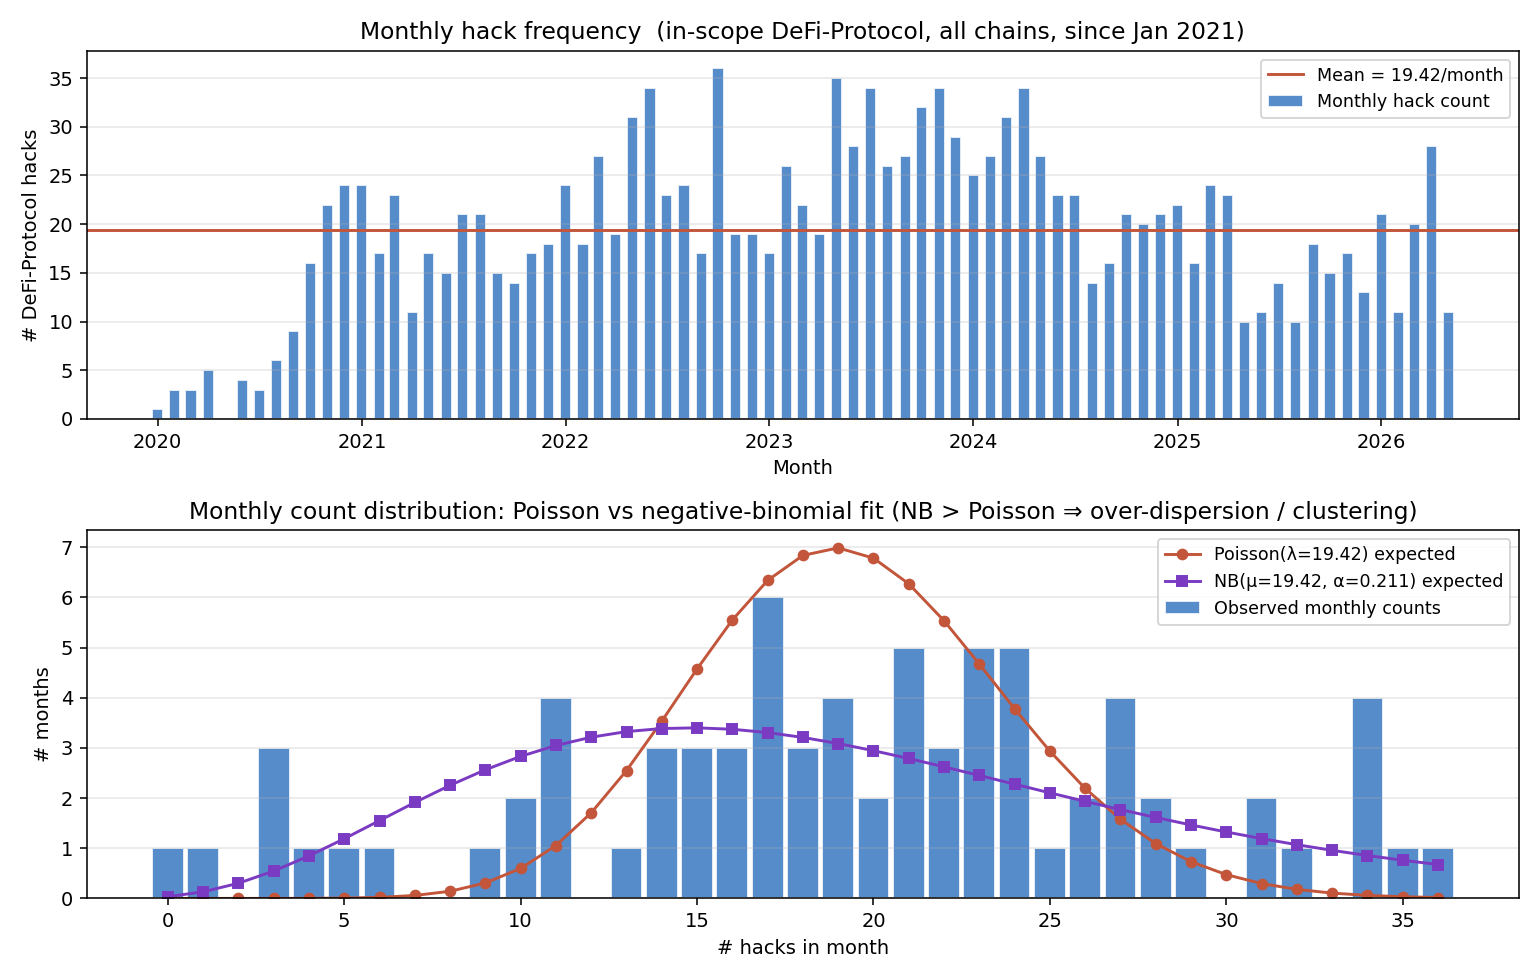
\includegraphics[width=0.92\linewidth]{r6_monthly_counts.png}
\caption{Top: monthly DeFi-Protocol event counts, 2016--2026.
Bottom: count distribution with Poisson and negative-binomial
overlays. Over-dispersion $D = s^2/\bar X = 3.9$ over the analysis
window is dominated by the 2020 regime shift but persists on the
stationary 2021--2026 subset.}
\label{fig:monthly}
\end{figure}


% ===========================================================================
\section{Capital requirements: an LDA for DeFi protocols}\label{sec:lda}
% ===========================================================================

\subsection{Why size capital, and against what}

Banks hold operational-risk capital against exactly the loss
process this paper has so far characterised: external attacks,
internal fraud, oracle / governance / mechanism abuse, deployment
errors, and infrastructure failures. Under Basel~III the
operational-risk capital requirement is the larger of the
Standardised Measurement Approach (SMA) charge and any Pillar~II
internal model the supervisor approves; the typical Tier-1 bank
holds operational-risk capital in the $8\text{--}15\%$-of-RWA
range, sized to absorb a 99.9\%-confidence one-year aggregate
operational-loss \citep{BCBS2017}.

DeFi protocols hold the same kind of buffer on-chain, under
governance control, sized by ad-hoc historical reasoning rather
than statistical modelling. The most visible examples are:

\begin{itemize}\setlength{\itemsep}{2pt}
  \item \textbf{Aave Umbrella} --- a multi-asset safety module
    (introduced in the Aave V3 ``Umbrella'' governance proposal,
    superseding the earlier single-asset Safety Module). Stakers
    deposit aTokens to cover bad-debt and shortfall events at the
    Aave market; the staked capital can be slashed to make depositors
    whole after an operational loss.
  \item \textbf{Liquity stability pool} --- LUSD holders deposit
    into a pool that absorbs liquidations and the gap between
    liquidated collateral and outstanding debt during volatile
    market events. The pool is sized by depositor demand, not by
    statistical loss modelling.
  \item \textbf{MakerDAO surplus buffer} --- a governance-controlled
    DAI reserve that absorbs unbacked debt before a debt auction is
    triggered; its target size (around DAI~250~m at the time of
    writing) is set by MIP-level governance vote rather than from
    a loss-distribution model.
  \item \textbf{Compound reserve factor} --- a per-market
    reserve accumulating a fraction of borrower interest, used
    historically to cover shortfalls. Sized as a fixed percentage
    of interest income rather than against a tail-loss target.
  \item \textbf{Curve crvUSD / GHO / sUSDe insurance funds} ---
    similar in spirit: protocol-owned reserves whose declared
    purpose is to absorb operational-risk and design-attack losses.
\end{itemize}

The empirical question is whether these reserves are adequately
sized, on the same statistical basis a bank supervisor would
apply. The loss-distribution-approach (LDA) machinery of
\citet{Cruz2002}, \citet{Chernobai2008}, and the OpRisk literature
provides the answer.

\subsection{Compound model}

In the standard operational-risk LDA framework, annual aggregate
loss is
\begin{equation}
S_{\text{year}} \;=\; \sum_{i=1}^{N} X_i,
\qquad N \sim \Poi(\hat\lambda_{\text{annual}}),
\qquad X_i \overset{\text{iid}}{\sim} F_X,
\end{equation}
where $\hat\lambda$ is the (per-sector or pooled) annual event rate
from \S\ref{sec:freq} and the severity $F_X$ is the piecewise
mixture of empirical-body and GPD-tail from \S\ref{sec:potgpd}.
We run $2\times 10^5$ independent simulated years per fit.

The resulting $\E[S]$, $\VaR_{99\%}$, and $\ES_{99\%}$ are the
pure-premium, regulatory-capital, and stress-capital numbers a
bank supervisor would compute --- and they are directly comparable
to the on-chain reserves listed above.

\subsection{Per-sector capital requirements}\label{sec:lda-sector}

The paper does not produce a pooled-DeFi capital number: the
severity and frequency parameters differ materially across
sectors (Lending fits $\hat\xi=0.93$, Stablecoin fits $0.30$ ---
pooling across them would mis-state both ends of the
distribution). Table~\ref{tab:lda-sector} reports the LDA output
by sector, using the per-sector POT-GPD fit (\S\ref{sec:potgpd})
and the per-sector annual event rate
(\S\ref{sec:per-sector-lambda}).

\begin{table}[h]
\centering
\small
\begin{tabular}{l r r r r r r r r}
\toprule
Sector & $n$ & $\hat\lambda$/yr & $\hat\xi$ & TVL (B) & $\E[S]$ bps & $\VaR_{99}$ bps & $\ES_{99}$ bps & $\ES_{99}$ USD \\
\midrule
Stablecoin   & 143 & 22.7 & 0.30 &   ---  &   ---   &     --- &    ---           &     --- \\
Lending      & 192 & 30.4 & 0.93 & 103.9  &   83    &   562   & \textbf{3{,}828} & 39.8~B  \\
DEX          & 274 & 43.4 & 0.62 &  15.2  &  180    &   922   & \textbf{2{,}013} &  3.1~B  \\
Yield        & 178 & 28.2 & 0.59 &  12.3  &  178    &   907   & \textbf{2{,}082} &  2.6~B  \\
Derivatives  &  44 &  7.0 & 1.58 &  71.0  &   ---   &     --- &    --- (n.c.)    &     --- \\
Bridge       &  93 & 14.7 & 0.60 &  50.1  &  141    &   981   & \textbf{2{,}141} & 10.7~B  \\
\bottomrule
\end{tabular}
\caption{Per-sector LDA capital requirements. ``TVL'' is the
trailing-365d sector average from the DefiLlama panel; bps figures
are relative to that sector's TVL. \textbf{Lending} carries the
largest absolute capital requirement (USD~40~B $\ES_{99\%}$
against USD~104~B TVL) and is the only sector whose $\hat\xi$ sits
close to the infinite-mean boundary; \textbf{Bridge, DEX, Yield}
fit $\hat\xi\in[0.59, 0.62]$ and produce capital requirements in
the $1{,}900$--$2{,}200$~bps-of-TVL band. \textbf{Stablecoin} fits
a markedly lighter tail ($\hat\xi=0.30$) and is omitted from the
LDA numerical column because the DefiLlama TVL panel for the
algorithmic-stablecoin bucket is not a credible denominator for
the universe of Stablecoin-sector OpRisk events (the panel
excludes the dominant centralised-collateralised stablecoin
issuers USDT/USDC by design); the severity fit is reported for
record. \textbf{Derivatives} ($n=44$, $\hat\xi=1.58$) is
sample-size-limited and produces a numerically unstable LDA in
the infinite-mean regime; the figure is omitted (``n.c.''~=~not
computed) and the sector is discussed qualitatively in
\S\ref{sec:pathology} below.}
\label{tab:lda-sector}
\end{table}

The $\ES_{99\%}$ bps figures in Table~\ref{tab:lda-sector} are
reported against sector TVL because that is the denominator
under which the LDA was simulated. The bound that matters
operationally is \emph{protocol} TVL --- a protocol cannot lose
more than its own users supplied --- so the bps ratio is intended
to be read as ``$\ES_{99\%}$ as a percentage of protocol TVL'' and
applied per-protocol in \S\ref{sec:protocol-adequacy}.
\emph{Bridge, DEX, and Yield} fit moderately-heavy OpRisk tails
and produce $\ES_{99\%}$ ratios in the $19$--$22\%$ band ---
broadly aligned with bank Tier-1 operational-risk capital ratios
($8$--$15\%$ of risk-weighted assets) once one adjusts for the
narrower scope of DeFi operational risk vs.\ a universal-bank
loss universe. \emph{Lending} is the outlier: $\hat\xi=0.93$, and
historical mega-events at the Vires Finance / Euler V1 / CREAM /
BonqDAO scale push the $\ES_{99}$ ratio to $\sim 38\%$ of
protocol TVL.

\subsection{Protocol-level adequacy: Aave, MakerDAO, Compound}\label{sec:protocol-adequacy}

The per-sector $\ES_{99\%}$-in-bps numbers in
Table~\ref{tab:lda-sector} translate mechanically into
\emph{protocol-level} capital targets by multiplying through the
protocol's individual TVL. We apply this to the three flagship
protocols that maintain explicit on-chain operational-risk
reserves --- Aave V3 (Lending), MakerDAO/Sky (a hybrid
stablecoin-issuer-plus-collateralised-debt-position venue that
behaves as a Lending sector exposure at the protocol-event level),
and Compound (Lending) --- and compare to the publicly-visible
size of those reserves. Protocol TVL figures are approximate
snapshots at the time of writing (May~2026); the calibration moves
mechanically as TVL moves.

\begin{table}[h]
\centering
\small
\begin{tabular}{l l r r r l}
\toprule
Protocol & Sector & TVL (B) & Modelled $\ES_{99\%}$ (B) & On-chain buffer & Coverage \\
\midrule
Aave V3   & Lending & $\sim 30$  & $\sim 11.5$ & Umbrella stake $\sim 0.3$~B & $\sim 3\%$  \\
MakerDAO  & Lending & $\sim 8$   & $\sim 3.1$  & Surplus buffer $\sim 0.25$~B & $\sim 8\%$  \\
Compound  & Lending & $\sim 3$   & $\sim 1.1$  & Per-market reserves $\sim 0.10$~B & $\sim 9\%$  \\
\bottomrule
\end{tabular}
\caption{Protocol-level operational-risk capital adequacy under
the Lending sector LDA. ``Modelled $\ES_{99\%}$'' is the
protocol's TVL multiplied by the Lending sector
$\ES_{99\%}/$TVL ratio of $3{,}828$~bps from
Table~\ref{tab:lda-sector}. ``On-chain buffer'' is the
publicly-visible safety-module / surplus-buffer / reserve
balance. ``Coverage'' is the buffer as a fraction of the modelled
$\ES_{99\%}$. Aave's Umbrella safety module (introduced in the
Aave V3 ``Umbrella'' governance proposal, superseding the
single-asset Safety Module) covers $\sim 3\%$ of the modelled
tail; MakerDAO's surplus buffer (DAI reserve that absorbs
under-collateralised vault losses before a debt auction) covers
$\sim 8\%$; Compound's per-market reserve factor covers
$\sim 9\%$. None of the three clears a credible bank-equivalent
operational-risk capital target. TVL and buffer figures are
approximate; the calibration is the mechanically transparent
piece.}
\label{tab:protocol-adequacy}
\end{table}

\emph{The headline reading.} None of the three flagship Lending
protocols is reserved against the modelled $99\%$-confidence
one-year tail event. Realised loss experience 2024--2025
(USD~1--2~B/yr DeFi-wide) sits in the body of the simulated
distribution and is comfortably absorbed by existing reserves;
the gap is in the tail. A Vires-Finance- or Euler-V1-class event
at the scale of supplied capital concentrated in any of these
three protocols would not be absorbed by the on-chain capital
stack and would impair user deposits.

\subsection{Pricing operational-risk insurance for protocols without buffers}\label{sec:insurance-pricing}

Aave, MakerDAO, Compound, and a handful of other established
protocols maintain explicit on-chain operational-risk reserves;
the vast majority of DeFi protocols do not. For those protocols
--- the long tail of mid- and small-cap Lending, DEX, Yield, and
Bridge pools that constitutes the bulk of the consolidated event
dataset --- the per-sector LDA output prices a stand-alone
\emph{protocol operational-risk insurance cover} on exactly the
same statistical basis.

The pure premium for a one-year cover with no deductible is, by
construction, the per-sector $\E[S]/$TVL ratio (``$\E[S]$ bps''
column of Table~\ref{tab:lda-sector}) applied to the covered
protocol's own TVL: $\approx 0.8\%/$yr for Lending, $\approx
1.4\%/$yr for Bridge, $\approx 1.8\%/$yr for DEX and Yield. A
risk-loaded premium --- the operationally relevant figure for a
cover writer who needs to hold capital against the cover itself
--- is the per-sector $\ES_{99\%}/$TVL ratio for a one-year cover
horizon, applied to the protocol TVL the writer is on the hook
for: the $19$--$38\%$-of-protocol-TVL band reported above. The per-sector LDA therefore produces
simultaneously (i) the target reserve size for self-insuring
protocols and (ii) the risk-loaded premium for externally-
insuring protocols. The two readings are equivalent: the
modelled $99\%$-confidence one-year operational-risk capital
requirement, expressed once as ``hold this much in your safety
module'' and once as ``pay this much premium per year'' against a
cover writer who does.

\subsection{The $\xi \geq 1$ pathology and the case for TVL truncation}\label{sec:pathology}

The Derivatives sector fit ($\hat\xi=1.58$, $n=44$) and to a
lesser extent the Lending fit ($\hat\xi=0.93$) sit close to or
above the infinite-mean boundary. Theoretically:
\begin{itemize}\setlength{\itemsep}{1pt}
  \item $\xi < 1$: $\E[X]$ finite.
  \item $\xi < 1/2$: $\Var(X)$ finite.
  \item $\xi \geq 1$: $\E[X] = \infty$.
\end{itemize}
In Basel-II operational risk this pathology is famous. Internal
LDA models produced regulatory capital charges so volatile and so
sensitive to single tail observations that the BCBS replaced
internal LDA with the Standardised Measurement Approach in 2017
\citep{BCBS2017}, abandoning the model class. The OpRisk-literature
remedy is \emph{severity truncation}: cap the tail at a plausible
per-event upper bound. The natural truncation point in DeFi is
\emph{per-protocol TVL} --- a protocol cannot lose more than its
own users supplied; the per-sector $\ES_{99\%}$-in-bps figure of
Table~\ref{tab:lda-sector} is therefore correctly read as a
\emph{ratio} applied to each protocol's individual TVL rather than
as an absolute aggregate against summed sector TVL. The Lending
headline $\ES_{99\%}=3{,}828$~bps figure is the credible
capital-sizing target at the protocol level; the Derivatives row
remains numerically unstable until the sample size grows, and is
treated qualitatively rather than as a capital number.

% ===========================================================================
\section{Discussion}\label{sec:discussion}
% ===========================================================================

\subsection{DeFi OpRisk, sized like a bank}

The central quantitative findings of the paper are summarised in
Tables~\ref{tab:lda-sector}--\ref{tab:protocol-adequacy}:
per-sector operational-risk capital requirements for DeFi
protocols, computed from the standard operational-risk LDA
framework that banking regulators apply to their AMA / SMA
Pillar~II calculations, and applied at the protocol level to the
three flagship Lending venues (Aave, MakerDAO, Compound). Read
those numbers the way a Tier-1 bank supervisor would read its own
OpRisk capital line.

The per-sector $\ES_{99\%}$ figures are reported as bps of
\emph{sector} TVL only because that is the denominator the LDA
sees during simulation; the operationally meaningful reading is
the same ratio applied to each individual protocol's TVL --- a
protocol cannot lose more than its own users supplied. For
\textbf{Bridge}, \textbf{DEX}, and \textbf{Yield}, the per-sector
$\ES_{99\%}$ ratio of $19$--$22\%$ of TVL translates into an
$\ES_{99\%}$ capital target of $19$--$22\%$ of any individual
protocol's own TVL --- broadly comparable to bank Tier-1 OpRisk
capital ratios ($8$--$15\%$ of risk-weighted assets) once one
accounts for the narrower scope of DeFi operational risk relative
to a universal bank's full loss universe. For \textbf{Lending}
the capital requirement is materially larger: $\ES_{99\%}\approx
38\%$ of protocol TVL, driven by the near-critical $\hat\xi=0.93$
tail and the existence of nine-figure historical losses (Vires
Finance, Euler V1, BonqDAO, CREAM). Applied at the protocol level
in Table~\ref{tab:protocol-adequacy}, none of Aave V3, MakerDAO,
or Compound clears more than $\sim 10\%$ of its protocol-level
modelled $\ES_{99\%}$ on the strength of its on-chain
operational-risk reserves alone. The modelled gap is the operational-risk capital
that the protocol's safety module, surplus buffer, or reserve
factor would need to grow into in order to be in the same
statistical regime as a Tier-1 bank's OpRisk capital.

\subsection{Where DeFi sits in the cross-field comparison}

Table~\ref{tab:crossfield} places the measured DeFi parameters
alongside published ranges for adjacent quantitative-risk literatures.

\begin{table}[h]
\centering
\small
\begin{tabular}{lccc}
\toprule
Process & Tail $\xi$ & Bound & Capital as \% of base \\
\midrule
Equity daily returns         & 0.2--0.4  & ---                  & 2--3\%                \\
Property / NatCat            & 0.5--1.0  & weather physics      & 0.3--1\% GWP          \\
Banking OpRisk (event-type)  & 0.85--1.4 & regulator + capital  & 8--15\% RWA (Tier 1)  \\
Cyber-breach losses          & 0.7--1.1  & ---                  & not regulated         \\
\textbf{DeFi-Lending}        & \textbf{0.93}      & protocol TVL & \textbf{$\ES_{99}\!\approx\!38\%$ protocol TVL} \\
\textbf{DeFi-Bridge / DEX / Yield} & \textbf{0.59--0.62} & protocol TVL & \textbf{$\ES_{99}\!\approx\!19\text{--}22\%$ protocol TVL} \\
\textbf{DeFi-Stablecoin}     & \textbf{0.30}      & protocol TVL & --- (TVL panel not credible) \\
\bottomrule
\end{tabular}
\caption{Cross-field summary. Read by sector: DeFi-Lending fits
just below the infinite-mean boundary and produces a capital
requirement comparable to or exceeding the bank Tier-1 ratio
applied to RWA; DeFi-Bridge, DEX, and Yield fit in the
moderate-OpRisk range; DeFi-Stablecoin fits markedly lighter. The
binding upper bound on a DeFi-protocol loss is \emph{protocol
TVL} --- a protocol cannot lose more than its own users supplied
--- not aggregate sector TVL; the per-sector
$\ES_{99\%}$-in-bps figures used as the right-hand column
translate mechanically into per-protocol capital targets via
each protocol's individual TVL (Table~\ref{tab:protocol-adequacy}).}
\label{tab:crossfield}
\end{table}

The cross-field reading lines up with a single conclusion: DeFi
operational risk \emph{can} be quantified on the same statistical
footing as banking OpRisk and \emph{should} be sized the same way.
The DeFi tail is no heavier than published Basel-II OpRisk fits
\citep{Moscadelli2004}.

\subsection{Why the heavy tail?}

Three structural features generate the per-sector severity tails
we measure.

\begin{enumerate}\setlength{\itemsep}{2pt}
  \item \textbf{Concentrated value behind a single point of failure.}
    Every protocol contracts its entire TVL pool to a piece of
    smart-contract code whose bug surface was fixed at deploy time,
    regardless of how much capital subsequently accumulates. There
    is no per-event regulatory cap, no insurance sublimit, no policy
    deductible --- only the protocol's own on-chain reserves.
  \item \textbf{Public mempool observability.} Attackers can read the
    same smart-contract bytecode as defenders, often with better
    tooling. Information asymmetry runs in the attacker's favour on
    reconnaissance, before flipping in the defender's favour only
    after the first event goes live.
  \item \textbf{Cross-protocol composability.} An exploit in
    protocol $A$ changes the on-chain conditions that determine the
    exploitability of protocol $B$ via shared oracles, shared
    liquidity pools, or shared synthetic assets. The resulting
    cross-protocol contagion is qualitatively visible in the
    rolling-intensity plots of \S\ref{sec:timeplot} and is the
    natural target of a separate Hawkes self-excitation analysis on
    the same dataset.
\end{enumerate}

The combination of these three features --- not any one in
isolation --- is what places DeFi-Lending in the upper part of the
banking-OpRisk distribution rather than in the moderately-heavy
NatCat / cyber range.

\subsection{Implications for DeFi stakeholders}

The numbers in Table~\ref{tab:lda-sector} translate into concrete
guidance for the three constituencies that hold the on-chain
capital infrastructure:

\paragraph{Protocol teams and DAOs.}
Treat the per-sector $\ES_{99\%}$ as a capital target, not a
forecast. Aave's Umbrella stake, MakerDAO's surplus buffer,
Compound's market reserves, and equivalents at Curve / Liquity /
Frax / GHO / sUSDe are the protocol-side equivalents of bank
operational-risk capital. Their adequacy can be assessed by
comparing pool size to the protocol's pro-rata share of the
sector $\ES_{99\%}$. Lending protocols in particular should
expect to hold safety-module capital at $5$--$10\%$ of supplied
TVL to be in the same regime as a Tier-1 bank's OpRisk capital
ratio; current Aave Umbrella stake of $\sim$USD~100--500~m against
$\sim$USD~30~B of supplied Aave TVL is two orders of magnitude
short of that target. Cross-protocol contagion --- visible in the
rolling-intensity plots and the natural target of a follow-up
Hawkes self-excitation analysis on the same dataset --- additionally
suggests that the windows after a peer-protocol event are
elevated-hazard periods during which deposit caps and upgrade
freezes function as the operational equivalent of bank monitoring
escalation.

\paragraph{Depositors and integrators.}
Users supplying capital to a protocol can read the sector
$\ES_{99\%}$ as the implied 1-in-100-year haircut their position
faces if the protocol's safety reserve is the only buffer. A
DeFi-Lending depositor at a protocol with no safety reserve
faces, on this estimate, $\sim 60\%$ of supplied capital at the
99\%-confidence one-year tail. A protocol with a safety reserve
sized to its sector share of $\ES_{99\%}$ reduces that haircut to
zero in expectation across the same tail; partial coverage moves
the haircut linearly. The capital-sizing framework gives a
quantitative basis for protocol selection that does not currently
exist in retail-grade DeFi risk dashboards.

\paragraph{Policy makers and supervisors.}
The Standardised Measurement Approach is the obvious analogue for
DeFi-protocol operational-risk regulation: a fixed
percentage-of-TVL capital charge with a multiplier indexed to
historical losses, low-touch in computation and high-touch in
disclosure. The Pillar~3 disclosure regime is also a clean fit:
mandatory reporting of event-level operational-risk loss data
already exists as a private initiative
(DefiLlama / SlowMist / de.fi) and would translate into a
regulated disclosure obligation with minimal new infrastructure.
The standardised loss-data feed is the precondition for any
industry-wide LDA modelling and for the credible capital-sizing
exercise this paper performs at the dataset level.

\subsection{Limitations}\label{sec:limits}

The calibration carries five caveats that an LDA-aware reader
should keep in mind.
\textbf{Censoring}: DefiLlama's hack ledger is well-curated for
material events but undoubtedly under-reports small losses (events
patched silently, near-misses, dust drains). This biases the body
of the severity distribution downward but is unlikely to affect
tail estimates.
\textbf{Cross-protocol attribution}: some events have an immediate
technical target distinct from the protocol whose balance sheet
carries the ultimate loss (Kelp/rsETH $\to$ Aave bad debt is the
salient case in our 2026 records). We follow the immediate-target
convention; readers interested in ultimate-loser attribution can
re-aggregate Bridge with downstream sectors in subsequent
analysis.
\textbf{Stationarity}: the 2020 regime shift drives the
cross-sector over-dispersion of monthly counts. We use the
full-window per-sector rate in the LDA; a non-stationary
background rate is a natural future extension.
\textbf{Independence across events}: the compound Poisson--GPD LDA
assumes per-sector iid event arrivals. The rolling-intensity plots
and the cross-sector monthly-count over-dispersion both flag
temporal clustering that violates this assumption; the resulting
LDA capital figures should be read as lower bounds on the joint
cross-sector tail, with a follow-up self-excitation analysis on
the same dataset necessary for a credible joint capital number.
\textbf{Recovery and net loss}: all figures in this paper are on
gross loss. Net of returned funds, the DeFi total is $\sim 6\%$
smaller; recovery is bimodal (almost-all or almost-none) and
statistically separable from the tail parameters.

% ===========================================================================
\section{Conclusion}\label{sec:conclusion}
% ===========================================================================

DeFi disintermediates financial services by outsourcing custody,
settlement, and counterparty credit risk to smart-contract code,
but operational risk remains in the system --- and has expressed
itself in aggregate gross losses of USD~11.2~B across 1{,}495
events on DeFi protocols since 2020. Banks size capital against
analogous losses under Basel~III; DeFi protocols maintain
functionally equivalent on-chain reserves (Aave Umbrella,
MakerDAO surplus buffer, Compound reserve factor) but those
reserves are sized today by governance vote rather than empirical
loss data. This paper performs the calibration.

Per-sector POT-GPD severity fits give $\hat\xi=0.93$ for Lending
(close to the infinite-mean boundary, statistically
indistinguishable from \citet{Moscadelli2004}'s canonical Basel-II
banking operational-risk range), $\hat\xi\in[0.59, 0.62]$ for
DEX, Yield, and Bridge, and $\hat\xi=0.30$ for Stablecoin.
Combining these severity tails with per-sector annual event rates
in a compound Poisson--GPD LDA Monte Carlo produces per-sector
$\ES_{99\%}$ ratios in the $1{,}900$--$3{,}800$-bps band
($19$--$38\%$ of protocol TVL, the binding upper bound on what a
single protocol can lose).

Applied at the protocol level, the implication is direct. Aave V3
($\sim$USD~30~B supplied lending TVL) carries a modelled
$\ES_{99\%}$ of $\sim$USD~11~B against an Umbrella stake currently
in the USD~100--500~m range --- coverage $\sim 3\%$ of the
modelled tail. MakerDAO ($\sim$USD~8~B TVL,
$\sim$USD~250~m surplus buffer) sits at $\sim 8\%$; Compound at
$\sim 9\%$. None of the three flagship Lending venues is
reserved against the modelled $99\%$-confidence one-year tail
event. Realised loss experience 2024--2025 sits comfortably in
the body of the distribution and is absorbed by existing reserves;
the gap is in the tail. For the long tail of DeFi protocols that
maintain no formal capital buffer, the same per-sector
$\ES_{99\%}$ ratios price a stand-alone operational-risk insurance
cover on the same statistical basis. The cross-protocol contagion
visible in the rolling-intensity plots warns that the per-sector
iid assumption underestimates joint tail risk across structurally
similar protocols, and is the natural target of a follow-up
self-excitation analysis on the same dataset.

% ===========================================================================
\section*{Reproducibility}
% ===========================================================================

The full data-collection and analysis pipeline, including the cached
raw source data, the consolidation logic, the inferential sector and
risk-category rule sets, and the analysis scripts that produce every
table and figure in this paper, is distributed as a reproducible
codebase. The pipeline runs deterministically on a fixed pseudorandom
seed. See the codebase README for the run-time orchestration: cached
raw source data, the canonical event master CSV, and the analysis
output JSON.

% ===========================================================================
% Bibliography (inline, no external .bib)
% ===========================================================================
\begin{thebibliography}{99}
\setlength{\itemsep}{2pt}

\bibitem[Sch\"ar(2021)]{Schar2021}
Sch\"ar, F. (2021).
Decentralized finance: On blockchain- and smart contract-based
financial markets.
\emph{Federal Reserve Bank of St.\ Louis Review}, 103(2), 153--174.

\bibitem[Aramonte et~al.(2021)]{Aramonte2021}
Aramonte, S., Huang, W., \& Schrimpf, A. (2021).
DeFi risks and the decentralisation illusion.
\emph{BIS Quarterly Review}, December 2021, 21--36.

\bibitem[Auer et~al.(2024)]{Auer2024}
Auer, R., Haslhofer, B., Kitzler, S., Saggese, P., \& Victor, F.
(2024). The technology of decentralized finance (DeFi).
\emph{Digital Finance}, 6(1), 55--95.

\bibitem[BlockSec(2026)]{BlockSec2026}
BlockSec (2026). Weekly Web3 Security Incident Roundups.
\url{https://blocksec.com/blog} (15 weekly posts ingested, accessed
2026-05-18).

\bibitem[DeFiHackLabs(2026)]{DeFiHackLabs2026}
SunWeb3Sec et~al.\ (2021--2026).
\emph{DeFiHackLabs: Reproduce DeFi hacked incidents using Foundry.}
GitHub repository, \url{https://github.com/SunWeb3Sec/DeFiHackLabs}
(accessed 2026-05-18).

\bibitem[Baldwin et~al.(2017)]{Baldwin2017}
Baldwin, A., Beres, Y., Duggan, G., Casassa Mont, M., Johnson, H.,
Middup, C., \& Shiu, S. (2017).
Contagion in cyber security attacks.
\emph{Journal of the Operational Research Society}, 68(7), 780--791.

\bibitem[BCBS(2006)]{BCBS2006}
Basel Committee on Banking Supervision (2006).
\emph{International Convergence of Capital Measurement and Capital
Standards: A Revised Framework, Comprehensive Version (Annex 9:
Detailed Loss Event Type Classification).}
Bank for International Settlements.

\bibitem[BCBS(2017)]{BCBS2017}
Basel Committee on Banking Supervision (2017).
\emph{Basel III: Finalising post-crisis reforms.}
Bank for International Settlements.

\bibitem[de.fi(2026)]{DeFiRektDb2026}
de.fi (formerly DeFiYield) (2026).
\emph{rekt-database.}
Paginated REST API at \texttt{https://api.de.fi/v1/rekt/list}; UI at
\texttt{https://de.fi/rekt-database}. Retrieved 2026-05-19.

\bibitem[SlowMist(2026)]{SlowMistHacked2026}
SlowMist Team (2026).
\emph{SlowMist Hacked.}
Public blockchain-event tracker at
\texttt{https://hacked.slowmist.io}. Retrieved 2026-05-19.

\bibitem[Bessy-Roland et~al.(2021)]{Bessy2021}
Bessy-Roland, Y., Boumezoued, A., \& Hillairet, C. (2021).
Multivariate Hawkes process for cyber insurance.
\emph{Annals of Actuarial Science}, 15(1), 14--39.

\bibitem[Chainalysis(2024)]{Chainalysis2024}
Chainalysis (2024).
\emph{The 2024 Crypto Crime Report.}
Chainalysis Inc.

\bibitem[Chernobai et~al.(2008)]{Chernobai2008}
Chernobai, A., Rachev, S. T., \& Fabozzi, F. J. (2008).
\emph{Operational Risk: A Guide to Basel II Capital Requirements,
Models, and Analysis.}
Wiley.

\bibitem[Clauset et~al.(2009)]{Clauset2009}
Clauset, A., Shalizi, C. R., \& Newman, M. E. J. (2009).
Power-law distributions in empirical data.
\emph{SIAM Review}, 51(4), 661--703.

\bibitem[Cope et~al.(2009)]{Cope2009}
Cope, E. W., Mignola, G., Antonini, G., \& Ugoccioni, R. (2009).
Challenges and pitfalls in measuring operational risk from loss
data.
\emph{Journal of Operational Risk}, 4(4), 3--27.

\bibitem[Cruz(2002)]{Cruz2002}
Cruz, M. G. (2002).
\emph{Modeling, Measuring and Hedging Operational Risk.}
Wiley.

\bibitem[Daian et~al.(2019)]{Daian2019}
Daian, P., Goldfeder, S., Kell, T., Li, Y., Zhao, X., Bentov, I.,
Breidenbach, L., \& Juels, A. (2019).
Flash Boys 2.0: Frontrunning, Transaction Reordering, and Consensus
Instability in Decentralized Exchanges.
\emph{IEEE Symposium on Security and Privacy.}

\bibitem[DefiLlama(2026)]{Defillama}
DefiLlama (2026). Public hack ledger and protocol catalog.
\url{https://api.llama.fi/hacks} (accessed 2026-05-16).

\bibitem[Donnelly \& Embrechts(2010)]{DonnellyEmbrechts2010}
Donnelly, C., \& Embrechts, P. (2010).
The devil is in the tails: Actuarial mathematics and the subprime
mortgage crisis.
\emph{ASTIN Bulletin}, 40(1), 1--33.

\bibitem[Dutta \& Perry(2006)]{DuttaPerry2006}
Dutta, K., \& Perry, J. (2006).
A tale of tails: An empirical analysis of loss distribution models
for estimating operational risk capital.
\emph{Federal Reserve Bank of Boston Working Paper.}

\bibitem[Edwards et~al.(2016)]{Edwards2016}
Edwards, B., Hofmeyr, S., \& Forrest, S. (2016).
Hype and heavy tails: A closer look at data breaches.
\emph{Journal of Cybersecurity}, 2(1), 3--14.

\bibitem[Eling \& Wirfs(2019)]{Eling2019}
Eling, M., \& Wirfs, J. (2019).
What are the actual costs of cyber risk events?
\emph{European Journal of Operational Research}, 272(3), 1109--1119.

\bibitem[Embrechts et~al.(1997)]{EmbrechtsKM1997}
Embrechts, P., Klüppelberg, C., \& Mikosch, T. (1997).
\emph{Modelling Extremal Events for Insurance and Finance.}
Springer.

\bibitem[de Fontnouvelle et~al.(2006)]{Fontnouvelle2006}
de Fontnouvelle, P., Jordan, J., \& Rosengren, E. (2006).
Implications of alternative operational risk modeling techniques.
In M. Carey \& R. Stulz (Eds.),
\emph{The Risks of Financial Institutions.} University of Chicago
Press, 475--512.

\bibitem[Hawkes(1971)]{Hawkes1971}
Hawkes, A. G. (1971).
Spectra of some self-exciting and mutually exciting point processes.
\emph{Biometrika}, 58(1), 83--90.

\bibitem[Heimbach et~al.(2024)]{Heimbach2024}
Heimbach, L., Vonlanthen, Y., Hara, T., \& Wattenhofer, R. (2024).
Quantifying the realized impact of MEV.
\emph{Financial Cryptography and Data Security.}

\bibitem[Helmstetter \& Sornette(2002)]{HelmstetterSornette2002}
Helmstetter, A., \& Sornette, D. (2002).
Subcritical and supercritical regimes in epidemic models of
earthquake aftershocks.
\emph{Journal of Geophysical Research}, 107(B10), 2237.

\bibitem[Hill(1975)]{Hill1975}
Hill, B. M. (1975).
A simple general approach to inference about the tail of a
distribution.
\emph{Annals of Statistics}, 3(5), 1163--1174.

\bibitem[ISO(2018)]{ISO2018}
International Organization for Standardization (2018).
\emph{ISO 31000:2018, Risk management --- Guidelines.}

\bibitem[Kismp(2026)]{Kismp2026}
Kismp123 et~al. (2020--2026).
\emph{DeFi-Security-Incident: A comprehensive reference of real-world
DeFi security incidents with root-cause analysis, attack flow, and PoC
code.}
GitHub repository, \url{https://github.com/kismp123/DeFi-Security-Incident}
(accessed 2026-05-18).

\bibitem[Maillart \& Sornette(2010)]{Maillart2010}
Maillart, T., \& Sornette, D. (2010).
Heavy-tailed distribution of cyber-risks.
\emph{European Physical Journal B}, 75(3), 357--364.

\bibitem[Moscadelli(2004)]{Moscadelli2004}
Moscadelli, M. (2004).
The modelling of operational risk: experience with the analysis of
the data collected by the Basel Committee.
\emph{Banca d'Italia Working Paper}, No.~517.

\bibitem[Arora et~al.(2026)]{Arora2026}
Arora, S., Li, Y., Feng, Y., \& Xu, J. (2026).
A risk scoring framework for critical infrastructure of
decentralized finance (DeFi).
\emph{Blockchain: Research and Applications}, article 100496.
\url{https://doi.org/10.1016/j.bcra.2026.100496}

\bibitem[Ogata(1988)]{Ogata1988}
Ogata, Y. (1988).
Statistical models for earthquake occurrences and residual analysis
for point processes.
\emph{Journal of the American Statistical Association}, 83(401),
9--27.

\bibitem[OpRisk Advisory \& Towers Perrin(2010)]{OpRiskAdvTowersPerrin2010}
OpRisk Advisory \& Towers Perrin (2010).
\emph{A New Approach for Managing Operational Risk: Addressing the
Issues Underlying the 2008 Global Financial Crisis.}
Society of Actuaries / Canadian Institute of Actuaries / Casualty
Actuarial Society.

\bibitem[Perez \& Livshits(2021)]{Perez2021}
Perez, D., \& Livshits, B. (2021).
Smart contract vulnerabilities: Vulnerable does not imply exploited.
\emph{USENIX Security Symposium.}

\bibitem[Pickands(1975)]{Pickands1975}
Pickands, J. (1975).
Statistical inference using extreme order statistics.
\emph{Annals of Statistics}, 3(1), 119--131.

\bibitem[Pisarenko \& Sornette(2003)]{Pisarenko2003}
Pisarenko, V. F., \& Sornette, D. (2003).
Characterization of the frequency of extreme earthquake events.
\emph{Pure and Applied Geophysics}, 160(12), 2343--2364.

\bibitem[Qin et~al.(2021)]{Qin2021}
Qin, K., Zhou, L., Livshits, B., \& Gervais, A. (2021).
Attacking the DeFi ecosystem with flash loans for fun and profit.
\emph{Financial Cryptography and Data Security.}

\bibitem[Rekt(2026)]{Rekt2026}
Rekt News (2020--2026). Rekt Leaderboard.
\url{https://rekt.news/leaderboard} (accessed 2026-05-18).

\bibitem[Romanosky(2016)]{Romanosky2016}
Romanosky, S. (2016).
Examining the costs and causes of cyber incidents.
\emph{Journal of Cybersecurity}, 2(2), 121--135.

\bibitem[Schuldenzucker et~al.(2017)]{Schuldenzucker2017}
Schuldenzucker, S., Seuken, S., \& Battiston, S. (2017).
Finding clearing payments in financial networks with credit default
swaps is PPAD-complete.
\emph{ITCS.}

\bibitem[Werner et~al.(2022)]{Werner2022}
Werner, S. M., Perez, D., Gudgeon, L., Klages-Mundt, A., Harz, D., \&
Knottenbelt, W. J. (2022).
SoK: Decentralized Finance (DeFi).
\emph{ACM Advances in Financial Technologies.}

\bibitem[Wheatley et~al.(2016)]{Wheatley2016}
Wheatley, S., Maillart, T., \& Sornette, D. (2016).
The extreme risk of personal data breaches and the erosion of
privacy.
\emph{European Physical Journal B}, 89(1), 7.

\bibitem[Zhou et~al.(2023)]{Zhou2023}
Zhou, L., Xiong, X., Ernstberger, J., Chaliasos, S., Wang, Z.,
Wang, Y., Qin, K., Wattenhofer, R., Song, D., \& Gervais, A. (2023).
SoK: Decentralized Finance (DeFi) Attacks.
\emph{IEEE Symposium on Security and Privacy.}

\end{thebibliography}

\end{document}
